\documentclass{article}

\usepackage{epsfig}
%\usepackage{cite}
\usepackage{bm}
\usepackage{amsmath}
\usepackage{times}
\usepackage{color}
% \usepackage{colortbl}
% \usepackage{rotating}
\usepackage{multirow}
\usepackage{url}
\usepackage{subfigure}
\usepackage{verbatim}
\usepackage{booktabs}
\usepackage[square,numbers,sort]{natbib}
\usepackage[pdfpagemode=UseOutlines,bookmarks=true,bookmarksopen=true]{hyperref}

\renewcommand{\textfraction}{0.1}
\newcommand{\D}{\displaystyle}
\newcommand{\T}{\mathrm}
\newcommand{\M}{\mathcal}
\newcommand{\dif}{\mathrm{d}}
\newcommand{\mm}{\mathbf{\mathcal{M}}}
\newcommand{\hl}{\vspace{6pt}\noindent\textbf}
\newcommand{\Si}{\Sigma}
\newcommand{\Sib}{\overline\Sigma}
\newcommand{\hs}{\hspace{0.1em}}

% \usepackage{fancyhdr}
% \fancypagestyle{plain}{%
% \fancyhf{}
% \renewcommand{\headwidth}{\textwidth}
% \renewcommand{\headrulewidth}{0pt}
% \renewcommand{\footrulewidth}{0.5pt}
% \setlength{\headsep}{5pt}
% }
% \pagestyle{plain}

\hyphenation{app-rox-ima-tion app-rox-ima-tions}

%--------DOCUMENT---------------------------------
\begin{document}

%\conferenceinfo{DAC 2008,}{June 8--13, 2008, Anaheim, California, USA.}
%\crdata{978-1-60558-115-6/08/0006}

\title{Virtual Prototyper (ViPro) User Guide}
\author{Satya Nalam}
%\author{Mihir Choudhury$^\dag$~~~~Vikas Chandra$^\ddag$~~~~Kartik Mohanram$^\ddag$~~~~Rob Aitken$^\dag$\vspace{2pt}\\
%$^\dag$Department of Electrical and Computer Engineering, Rice University, Houston\vspace{2pt}\\
%$^\ddag$ARM Inc., San Jose\vspace{2pt}\\
%\{mihir,kmram\}@rice.edu~~~~\{vikas.chandra,raitken\}@ufl.edu
%\author{Mihir Choudhury and Vikas Chanda and Kartik Mohanram and Rob Aitken\vspace{2pt}\\
%Department of Electrical and Computer Engineering, Rice University,
%Houston\vspace{2pt}\\
%\url{{mihir,kmram}@rice.edu}
%}

\maketitle
\section{About this document}
This document is a frequently updated user-guide for ViPro. While ViPro is still under construction, it will keep changing to reflect and document the current state of work.

\subsection{What is ViPro?}
ViPro is a technology-agnostic prototyping and design space exploration tool for SRAM. The primary input is a specification of the memory (e.g. capacity, word-size, technology, supply voltage). The primary output is a ``somewhat optimized" SRAM prototype (e.g. schematic, layout, gds) composed of periphery from the built-in library. The SRAM is not truly optimal since the number of knobs/variables for optimization is limited to make the problem manageable. A single-bank architecture is assumed (described in section ~\ref{arch}). In addition, ViPro will also allow easy design space exploration by allowing the user to specify custom periphery (to various degrees of detail - e.g. preliminary E-D data to completed designs) and generate a re-optimized prototype.

\subsection{Current state of ViPro}
The working of ViPro can be broadly divided into three main steps - E-D characterization of SRAM components, optimization and prototype generation. The characterization step is completed in this version, with frameworks for optimization and prototype generation in place. Also completed is a full schematic generator that can be used independently of ViPro to generate a full SRAM schematic in any technology, provided correct sizing and other parameters. ViPro is currently similar to CACTI in that it can give the energy per access and maximum frequency/access time for a given SRAM configuration. It also gives the E-D breakup among different components of the SRAM (e.g. Bitlines, decoder etc.). However, it is slower as it is simulation based and technology specific.

The E-D characterization data will be fed to a convex optimizer to generate the optimal values of the knobs. These values will then be used by the prototype generator (e.g. compiler) to build the SRAM using SKILL for schematics and PyCell for layout. The characterization itself is done by TASE (separate user guide available).

\section{Quick Start}

\subsection{Insructions}
These steps should help you get setup with ViPro. The instructions are for a linux machine.
\begin{description}
\item \textbf{Step 1:} Check out the TASE and ViPro to your workspace. You need to have a sub-version account setup. Sub-version help is available on the UVA ECE wiki.

\% mkdir /some/work/dir/vipro

\% cd /some/work/dir/vipro

\% svn checkout \$SVNROOT/SRAM\_TOOL/trunk

\% cd /some/work/dir/tase

\% svn checkout \$SVNROOT/SRAM\_TOOL/branches/TASE

\item \textbf{Step 2:} Set up Cadence environment.

\% . cadence-ic15141

\item \textbf{Step 3:} Configure user inputs in configuration/user.m and configuration/bitcellSizes.m. Bitcell generator settings can be made in configuration/cellgen.ini.

\begin{itemize}

\item The following parameters are defined in user.m.
\begin{enumerate}
\item technology - The string identifying the pdk. This should have a corresponding .ini file in the template directory. For example, if Technology=`ptm65', ensure that there is a RVPtpl\_ptm65.ini in the template/ directory.
\item wdef = default device width.
\item memSize - Memory size in bits.
\item arbits - Number of row address bits - will be log2(no: of rows)
\item acbits - Number of col address bits - will be log2(no: of cols)
\item wordSize - Size of the word in bits.
\item vdd, vsub - Nominal supply V$_\text{DD}$ and PMOS bulk V$_\text{DD}$.
\item temp - Temperature.

\item width - width of the bitcell in metres.
\item height - height of the bitcell in metres. Width and height of the bitcell need to be specified if using a custom bitcell (e.g. cell generator not invoked)

\item global/local/interMtl - type of metal for global, local and intermediate level interconnect. Can be either `cu' or `al'.

\item global/local/interParams - width, space, thickness, height, and dielectric constant for various levels of interconnect. To use default values built into the interconnect model, leave the parameters as zeros. Otherwise, custom dimensions can be specified in microns.

\item getMetrics - A boolean flag that is set to 1 if ViPro is being used only to estimate energy and delay for a particular configuration. The optimization related inputs will be ignored in that case. If getMetrics is 0, the optimization related inputs are also considered.

\item rows - Number of rows.
\item cols - Number of columns (= memSize(fixed)/rows).
\item wnio - Device widths for Tristate inverter in IO block
\item decStages - Number of predecode buffer and WL buffer stages respectively

\item tasePath - Absolute path for the location of TASE - should be of the form /some/work/dir/tase
\end{enumerate}

\item rows, wnio, and decStages are the current set of optimization knobs with respect to which characteristic sims are run in TASE. This set of knobs can be expanded along with potential new characterization sims in TASE corresponding to those knobs.

\item Constraints on Noise margin, I$_\text{READ}$, and bitcell area are specified for the bitcell generator in cellGen.ini. The bitcell generator has not been developed/maintained recently while the rest of ViPro has been changing and may need some testing and debugging before it is functional again.

\item The bitcell device sizes can be specified in bitcellSizes.m if the bitcell generator is not run and a foundry bitcell is used.

\end{itemize}


\item \textbf{Step 4:} Execute ViPro from the device/BIN directory

\% cd device/BIN

\% perl ViPro.pl --flag1 --flag2 ...

The various flags that can be used are
\begin{itemize}
\item --cellGen       - Run bitcell generator

\item --char          - Run the characterization (TASE) step. This is done at least once whether performing optimization or using in the get metrics mode.

\item --opt           - Run optimization engine.Currently inactive.

\item --compiler      - Run technology agnostic memory compiler (schematic and layout generator). Currently the generator resides in the compiler/ directory but is not callable yet from ViPro.pl. It also needs an optParams.txt file to be present in files/. This file is created manually but will eventually come from the optimizer output. See section~\ref{sec:compiler} for more info on this option.

\item --genCustom     - Only generate custom specified schematics and layout. Useful for just generating a completely specified memory skipping the characterization and optimization part. A files/sizes.txt file needs to be specified by the user.

\item --h,--help      - Display this help message

\item --quiet	      - Reduce the verbosity of the screen output

\item --clean         - Remove files/ directory prior to starting a new run of ViPro.pl
\end{itemize}
For a particular step to be executed, the corresponding flag must be specified. For instance, TASE does not run if --char is not specified in the command line arguments to ViPro.pl. The flags are case-insensitive and can be used with a single hyphen as well.

\end{description}

\textbf{NOTE:}
The examples in the quickstart instructions are currently for a user at UVA. Path names, environment setup etc. may change for an external user.

\subsection{Example run}
This is a walk-through example using the IBM 65 technology.

\begin{description}
\item Step 1: Setup the environment
\item Step 2: cd path-to-tool/device/BIN
\item Step 3: perl ViPro.pl --clean --char
\item Step 4: The breakdown of E,D numbers and Energy per accesss, max frequency will be in path-to-tool/files/debug*.txt and path-to-tool/files/topMetrics.txt.
\end{description}

The screen output looks like:
\begin{verbatim}
: /scratch/svn2u/ViPro_release/trunk/device/BIN $ perl ViPro.pl --clean --char
VIPRO:Checking sanity of user inputs
VIPRO:Getting Metal parasitic values for 'ibm65'
	
	  	     < M A T L A B (R) >
	   Copyright 1984-2010 The MathWorks, Inc.
	Version 7.10.0.499 (R2010a) 64-bit (glnxa64)
	  	      February 5, 2010


  To get started, type one of these: helpwin, helpdesk, or demo.
  For product information, visit www.mathworks.com.
 
VIPRO:Running Gate capacitance characterization for ibm65
VIPRO:Running characterizer
 new2tpl
  Initializing test: RVP_Gate_Capacitance
 tpl2scs
  Building test: RVP_Gate_Capacitance
 ocn2out
  Executing test: RVP_Gate_Capacitance
 dat2img
  Building graphical data for: RVP_Gate_Capacitance
  Compiling global image sets
Skipping img2pdf

Build complete for:   RVP_Gate_Capacitance


                    < M A T L A B (R) >
          Copyright 1984-2010 The MathWorks, Inc.
        Version 7.12.0.635 (R2011a) 64-bit (glnxa64)
                       March 18, 2011

 
  To get started, type one of these: helpwin, helpdesk, or demo.
  For product information, visit www.mathworks.com.

VIPRO:Running characterization for user configuration
VIPRO:Running characterizer
 new2tpl
  Initializing test: RVP_Ileak_PU
  Initializing test: RVP_Ileak_PD
  Initializing test: RVP_Ileak_PG
  Initializing test: RVP_DFF
  Initializing test: RVP_Inv_LEparams
  Initializing test: RVP_bufChains
  Initializing test: RVP_TIMING
  Initializing test: RVP_CD
  Initializing test: RVP_SA
  Initializing test: RVP_IO
  Initializing test: RVP_Decoder
 tpl2scs
  Building test: RVP_Ileak_PU
  Building test: RVP_Ileak_PD
  Building test: RVP_Ileak_PG
 scs2out
  Executing test: RVP_Ileak_PU
  Executing test: RVP_Ileak_PD
  Executing test: RVP_Ileak_PG
 out2dat
  Reading data from: RVP_Ileak_PU
   Extracting: dc.dc
  Reading data from: RVP_Ileak_PD
   Extracting: dc.dc
  Reading data from: RVP_Ileak_PG
   Extracting: dc.dc
 tpl2scs
  Building test: RVP_DFF
  Building test: RVP_Inv_LEparams
  Building test: RVP_bufChains
  Building test: RVP_TIMING
  Building test: RVP_CD
  Building test: RVP_SA
  Building test: RVP_IO
  Building test: RVP_Decoder
 ocn2out
  Executing test: RVP_DFF
  Executing test: RVP_Inv_LEparams
  Executing test: RVP_bufChains
  Executing test: RVP_TIMING
  Executing test: RVP_CD
  Executing test: RVP_SA
  Executing test: RVP_IO
  Executing test: RVP_Decoder
 dat2img
  Building graphical data for: RVP_Ileak_PU
  Building graphical data for: RVP_Ileak_PD
  Building graphical data for: RVP_Ileak_PG
  Building graphical data for: RVP_DFF
  Building graphical data for: RVP_Inv_LEparams
  Building graphical data for: RVP_bufChains
  Building graphical data for: RVP_TIMING
  Building graphical data for: RVP_CD
  Building graphical data for: RVP_SA
  Building graphical data for: RVP_IO
  Building graphical data for: RVP_Decoder
  Compiling global image sets
Skipping img2pdf

Build complete for:    RVP_Ileak_PU RVP_Ileak_PD RVP_Ileak_PG  RVP_DFF 
RVP_Inv_LEparams RVP_bufChains RVP_TIMING RVP_CD RVP_SA RVP_IO RVP_Decoder
VIPRO:Getting E and D for user-specified SRAM configuration
	
	              < M A T L A B (R) >
	    Copyright 1984-2010 The MathWorks, Inc.
	 Version 7.10.0.499 (R2010a) 64-bit (glnxa64)
	               February 5, 2010


  To get started, type one of these: helpwin, helpdesk, or demo.
  For product information, visit www.mathworks.com.
\end{verbatim}

The following files can now be found in path-to-tool/files:

\begin{verbatim}
: /scratch/svn2u/ViPro_release/trunk/device/BIN $ ls ../../files/
debugDelayRd.txt  debugDelayWrt.txt  debugEnergyRd.txt  debugEnergyWrt.txt 
parasitics.txt  topMetrics.txt
\end{verbatim}

These contain the breakdown of energy and delay. For example:
\begin{verbatim}
: /scratch/svn2u/ViPro_release/trunk/files $ cat debugEnergyWrt.txt 
Decoder(erowdec) = 1.177766e-12
IO(eio) = 1.718782e-12
CD(ecd) = 2.005102e-12
SA(esach) = 3.807166e-13
Bitcell(ebcwr) = 3.350314e-13
Timing(etmng) = 6.561755e-13
Leakage(elkg) = 3.098865e-17
Energy per write = 6.273604e-12
\end{verbatim}

\section{Tool Flow}
\label{RVP}
The executable to run ViPro is ViPro.pl in device/BIN. This section describes ViPro.pl in detail. The tool flow can be broadly divided into the following stages. Each stage can be enabled by providing the corresponding flag in the argument list for ViPro.pl.

1. Bitcell Generation

2. Characterization

3. Optimization

4. Schematic and Layout Generation

\subsection{Bitcell Generation}
If --cellGen is specified in the arguments, the bitcell generator generates optimal bitcell device sizes based on user-specified area, I$_\text{READ}$ and noise margin constraints and writes it to a file called ``range.final" along with other outputs. The device size data (in lambda units) is parsed from this file by \textbf{formatCGOutput.pl} and written to a file called ``cellGenOutput". Finally, the sizes are converted to absolute units in matlab-compatible format by \textbf{convert.m}. The final device sizes are output to ``bitcellsizes.m".

\subsection{Characterization}
The characterization stage is enabled by the --char flag and can be divided into the following stages:
\begin{enumerate}
\setlength{\itemsep}{0cm}
\setlength{\parskip}{0cm}
\item Metal parasitic estimation
\item Gate capacitance estimation
\item SRAM leaf cell E-D characterization or estimation for a fixed configuration 
\end{enumerate}

The technology node is determined from the user configuration file (configuration/user.m). This is used to determine the local, intermediate, and global interconnect resistance and capacitance parasitics using the extended PTM interconnect model defined in InterconnectCap.m. The values are determined by getParasitics.m and written to the temporary work directory (files/) in parasitics.txt.

Next, the gate capacitance is determined using TASE through the RVP\_Gate\_Capacitance test. For this step, first a .ini file is created to run this test from the corresponding template (RVPtpl) file. The user needs to ensure that the sweep range (e.g. gcap\_start, gcap\_stop) for the gate capacitance estimation is sufficient. If it is not, ViPro will fail and prompt the user to adjust this range so that the gate capacitance can be estimated within the tolerance specified (tol parameter in the .ini file).

The metal and gate capaciance values determined above are then appended to the .ini file. Finally, TASE is invoked to run the E-D characterization of the leaf cells. Before TASE is invoked, the bitcell sizes and the tests below are appended to the .ini template file:

\begin{itemize}
\item RVP\_Ileak\_PU - bitcell pullup leakage
\item RVP\_Ileak\_PD - bitcell pulddown leakage
\item RVP\_Ileak\_PG - bitcell passgate leakage
\item RVP\_DFF - DFF Delay
\item RVP\_Inv\_LEparams - Inverter logical effort parameters
\item RVP\_bufChains - Timing block buffer chain Power,Delay for horizontal control signals.
\item RVP\_Decoder - Decoder Power, Delay
\item RVP\_CD - Column Mux Power, Delay
\item RVP\_SA - SA Power, Delay
\item RVP\_IO - IO Power, Delay
\item RVP\_TIMING - Timing block Power, Delay
\end{itemize}

The characterization data is output in data*.txt. For the decoder it is in output\_\textless no: of address bits\textgreater. The simulation output can be examined in device/BIN/\textless user-id\textgreater /\textless test-name\textgreater.

\subsubsection{Getting metrics for a given configuration}
If the getMetrics flag in the user configurations file is set to 1, the tool determines the energy and delay breakdown among different components for the given configuration and also the total energy per access and maximum frequency of operation based on the calculated delays. Note that these metrics are for the nominal case with no variations impact considered. If this flag is used, then the characterization sweeps in the previous sections reduce to the simulation of a single user-specified configuration.

ViPro.pl first invokes getMetrics.m. This in turn invokes the getEnergy and getDelay functions, each of which instantiate the top-level SRAM object (described in~\ref{model}) and call its energy and delay methods respectively.

\subsection{Optimization}
The user can now either use ViPro to estimate the top-level metrics for a given configuration or allow the tool to generate an optimized SRAM configuration.

\subsection{Schematic and Layout Generation}
\subsubsection{Schematic Generator}
Full SRAM schematic generation starting from basic gates can be done for any technology. This module takes 3 inputs. These are as follows.
\begin{itemize}
\setlength{\itemsep}{0cm}
\setlength{\parskip}{0cm}
\item minSizes.txt - The main wrapper input file that contains the minimum/default width and length specifications for the nmos and pmos devices.
\item inputs.txt - The library name, technology details and top-level architectural specs (e.g. rows, cols, word-size) are specified in this file. 
\item sizes.txt - Outputs of the optimization - optimal device sizes, number of buffer stages etc. are specified in this file. These values override the defaults in the generator (typically minimum sizes for inverters and logical-effort based sizing for larger gates).
\end{itemize}

Currently these files are manually created and the schematic generator is manually called from the icfb main window. The eventual goal is for them to be automatically generated and for the generator to be automatically called from ViPro.pl. A description of the SKILL functions used by the schematic generator can be found in doc/userGuides/GeneratorFunctionList.pdf. 

\subsubsection{Layout Generation}


\begin{comment}
The bitcell characterization data is written to ``calcParams.m". The bitcell dimensions (e.g. width and height) are estimated using \textbf{getCellDimensions.m} that calls the area function and appends it to calcParams.m. This file is then combined with the user defined parameters in user.m to create a consolidated configuration file called ``constructor.m" in the model/ directory.

\subsection{Optimization}
The optimization variables are currently the number of rows (NR) and columns (NC) of the array. A brute force search that examines the energy and delay for the SRAM for several configurations is done to determine the optimal configuration that satisfies the user-specified constraints, while minimizing either energy or delay. Energy and Delay are calculated using the TASE output and the SRAM model described in section \ref{model}.

\subsection{Result Generation}
The optimization output will be used to generate pareto E-D curves, break-down of energy and delay among various SRAM components. Eventually, it will be used to generate actual schematics and layout for the optimal prototype.
\end{comment}

\section{Tool Structure}  
ViPro has the following sub-directories.
\begin{itemize}
\setlength{\itemsep}{0cm}
\setlength{\parskip}{0cm}
\item bin
\item cellGen
\item compiler
\item configuration
\item doc
\item model
\item files
\end{itemize}

\subsection{bin}
The bin directory contains a bunch of .pl files. These are described below-
\begin{itemize}
\setlength{\itemsep}{0cm}
\setlength{\parskip}{0cm}
\item ViPro.pl - The top-level wrapper script for ViPro that runs the entire flow from Characterization to optimization to prototype generation
\item char.pl - Characterization related helper functions
\item compiler.pl - Layout/schematic generation related helper functions.
\item optimizer.pl - Optimization related helper functions.
\item user.pl - Helper functions related to parsing user inputs.
\end{itemize}

\subsection{cellGen}
The cellGen directory contains following scripts and functions pertaining to the bitcell generator-
\begin{itemize}
\setlength{\itemsep}{0cm}
\setlength{\parskip}{0cm}
\item area.m - function to estimate bitcell dimensions and area.
\item cellGen.pl - Main bitcell generator that determines optimal bitcell sizes based on noise margin, I$_\text{READ}$ and area constraints.
\item formatCGOutput.pl - Parses the raw cellGen.pl output to generate the intermediate ``cellGenOutput".
\item convert.m - Generates the final ``bitcellSizes.m" from intermediate ``cellGenOutput".
\end{itemize}

The following intermediate results and logs are also found in this directory-
\begin{itemize}
\setlength{\itemsep}{0cm}
\setlength{\parskip}{0cm}
\item matlab.log - Execution log for the .m files
\item bitcellSizes.m - The generated final bitcell device size descriptor
\item area\_results, w\_results, h\_results - area, width, and height of the bitcell calculated by cellGen.pl in lambda units
\item range.init - Intermediate file containing the range of bitcell device sizes to be searched; keeps shrinking till the optimal bitcell configuration is determined.
\end{itemize}

\subsection{compiler}
The compiler directory is currently a place-holder for the automatic schematic generation and layout scripts in SKILL and/or PyCell, that will take the optimization output and generate schematics and layout for the SRAM prototype.

\subsection{configuration}
The configuration directory provides the user interface for ViPro. The user can enter top-level SRAM specifications such as technology, V$_\text{DD}$ etc., and constraints on energy, delay, noise margins etc. in various configuration files listed below.
\begin{itemize}
\setlength{\itemsep}{0cm}
\setlength{\parskip}{0cm}
\item bitcellSizes.m - Foundry/custom bitcell sizes can be provided here if the generator is not used.
\item user.m - Top-level specifications for the SRAM
\item cellGen.ini - Noise margin, I$_\text{READ}$, area constraints for bitcell generator
\item components - This file lists any additional TASE templates that need to be characterized other than the ones in the library. This is useful, for example, when the user wants to characterize a new circuit for an SRAM periphery component.
\end{itemize}

The user/ and sizes/ directory provide example bitcellSizes.m and user.m files for different technologies.

\subsection{doc}
This directory contains a comprehensive documentation for ViPro and the latex source code for it.

\subsection{model}\label{model}
The model directory contains the Hierarchical SRAM model in Matlab and the optimization code that uses TASE output to determine the optimal SRAM prototype. The files/directories that make up the model are briefly described below.
\begin{itemize}
%\setlength{\itemsep}{0cm}
%\setlength{\parskip}{0cm}
\item @SRAM\_Component - Abstract base class in Matlab that defines common properties and methods for different SRAM components. For example, properties such as technology, rows, columns, word size etc. are defined in the class. All other classes are inherited classes from the SRAM\_Component class

\item @SRAM\_Bitcell - Bitcell class. No local properties currently defined. Energy and delay methods (`E' and `D') defined which use the TASE output (that measures power/delay for a single bitcell/column). Energy contributed by all bitcells is calculated.

\item @SRAM\_CD - Column Mux class. The device sizes of the CD circuit are defined as local properties.

\item @SRAM\_Decoder - Decoder class

\item @SRAM\_IO - IO class. 

\item @SRAM\_SA - SA class. Device sizes of the SA are defined as local properties.

\item @SRAM\_Timing - Timing block class.

\item @SRAM\_Top - SRAM class that defines the top-level of the SRAM. The leakage of the bitcell devices, and objects of each component class (e.g. IO, CD, SA, Decoder, Bitcell, and Timing) are defined as local properties. The energy and delay model is implemented in this class. The energy and delay functions defined in the SRAM\_Top class call the corresponding functions of the component objects and estimate the energy and delay/fmax for the SRAM as described in section~\ref{model}.
\end{itemize}
In addition, each class has a constructor that initializes the properties of the class. The component class constructors first reference the super-class constructor (e.g. constructor of the SRAM\_Component class) to initialize the global parameters.

\subsection{files}
The files directory contains intermediate files and output files generated by ViPro. The following files are generated:

\begin{enumerate}
\setlength{\itemsep}{0cm}
\setlength{\parskip}{0cm}
\item parasitics.txt - metal parasitics for local, intermediate and global interconnect generated using the InterconnectCap fucntion in the model/directory.
\item debugXY.txt - where X refers to either energy or delay, Y refers to read or write. This file provides the total E,D and breakup among the various SRAM components for the given user configuration/
\item topMetrics.txt - The top-level metrics - worst case energy per access and maximum frequency of operation can be found in this file.
\end{enumerate}

\section{SRAM Architecture}
\label{arch}
ViPro assumes a single-bank architecture (Figure~\ref{fig:arch}),with a conventional 6T bitcell. The model used for determining the energy per access and minimum cycle time is based on this architecture. Larger memory capacities are usually organized in a multiple bank architecture, which is out of the scope of the current implementation of ViPro. Each SRAM component in the single-bank architecture is described below in the following sub-sections.

\begin{figure}[htb]
  \centering
  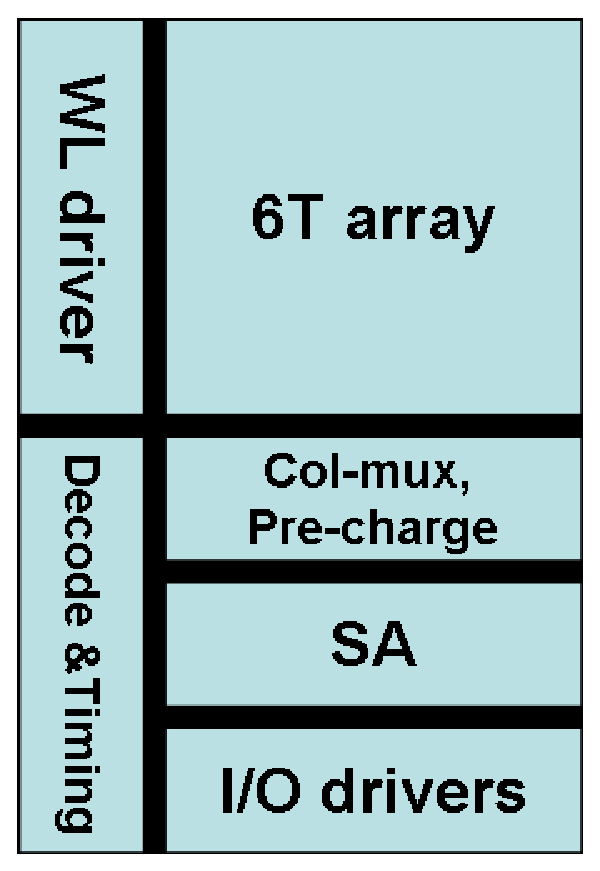
\includegraphics[scale=0.5]{Vipro_arch}
\vspace{-5pt}
  \caption{Single-bank SRAM architecture assumed by ViPro.}
  \label{fig:arch}
\vspace{-5pt}
\end{figure}

\subsection{Decoders and WL Driver}
The WL Driver assumed by ViPro (Figure~\ref{fig:wld})is a generic via-programmable circuit that can drive 8 WLs. It consits of a 2-input And, a 2-input Nand, and an inverter that drives the WL to the bitcells. The  Nand and And gates combine the pre-decoded signals to select a single WL. By connecting the inputs of the And gate to different combinations of the pre-decode signals (PRE8\_6 and PRE5\_3), different sets of 8 WLs can be driven. This structure enables only a single pre-decode (3 to 8) in the timing block (Figure~\ref{fig:tmg}) to be used for any number of rows, narrowing the optimization problem for the decoder to a single structure. The programmability of the WL driver also has potential benefits for schematic and layout automation.

\begin{figure}[htb]
  \centering
  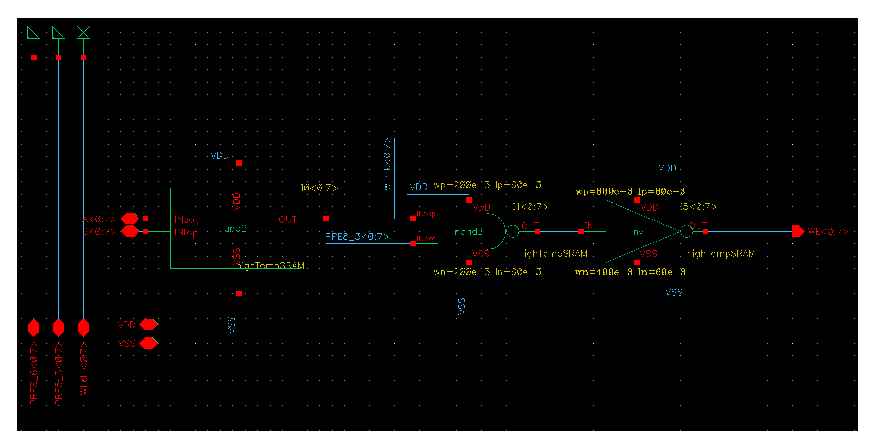
\includegraphics[scale=0.7]{WLD}
\vspace{-5pt}
  \caption{Via-programmable wordline driver in the ViPro architecture (zoom in for a clearer view).}
  \label{fig:wld}
\vspace{-5pt}
\end{figure}

\begin{figure}[htb]
  \centering
  \includegraphics[scale=0.5]{Vipro_row}
\vspace{-5pt}
  \caption{Timing block showing the predecode and the WL Driver.}
  \label{fig:tmg}
\vspace{-5pt}
\end{figure}

\subsection{CD}
The CD (Figure~\ref{fig:cd}) is composed of the BL precharge and equalize transistors, and the column-mux transmisssion gate. The figure shows a CD that uses a column-mux of 4. In general, a larger column-mux (e.g. 8) can be used for all cases, with the unused outputs of the decoder left floating. This also narrows the optimization problem.
\begin{figure}[htb]
  \centering
  \includegraphics[scale=0.8]{CD}
\vspace{-5pt}
  \caption{Column Mux circuit.}
  \label{fig:cd}
\vspace{-5pt}
\end{figure}


\subsection{SA}
The SA (Figure~\ref{fig:sa}) is composed of a differential voltage SA, a nand-based SR output latch, and precharge and equalize PFETS for the SA input nodes -  the muxed-out BLs (RDWR and NRDWR). The SA inputs are also connected to the write drivers (tri-state inverters) in the IO circuit.

\begin{figure}[htb]
  \centering
  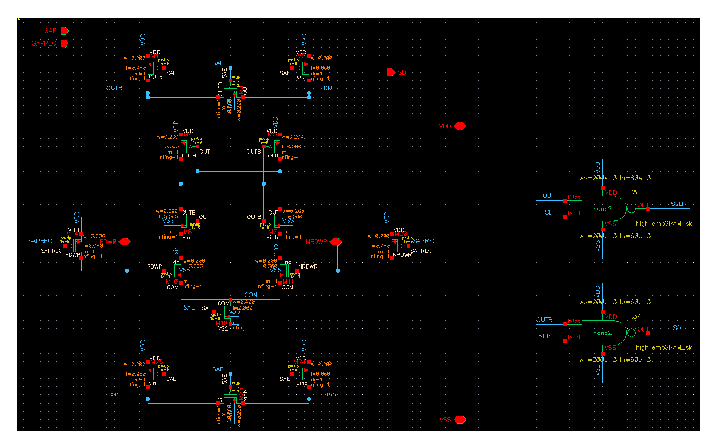
\includegraphics[scale=1.0]{SA}
\vspace{-5pt}
  \caption{Sense Amp circuit.}
  \label{fig:sa}
\vspace{-5pt}
\end{figure}

\subsection{IO}
The IO (Figure~\ref{fig:io}) consists of a flip-flop for the SA output during a read, and another one for the data input during a write. It also has tri-state inverters to drive the data to the bitlines, that get enabled during a write.

\begin{figure}[htb]
  \centering
  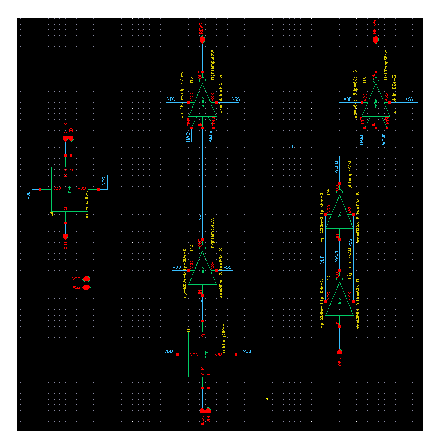
\includegraphics[scale=0.7]{IO}
\vspace{-5pt}
  \caption{Data Input and Output driver circuits. }
  \label{fig:io}
\vspace{-5pt}
\end{figure}

\subsection{Timing}
The precise timing block design varies from technology to technology depending on design constraints, capacitance of the control wires that need to be driven, etc. The basic functionality of the timing block and the control signals it drives is captured in Figure~\ref{fig:tmgblk}. 

\begin{figure}[htb]
  \centering
  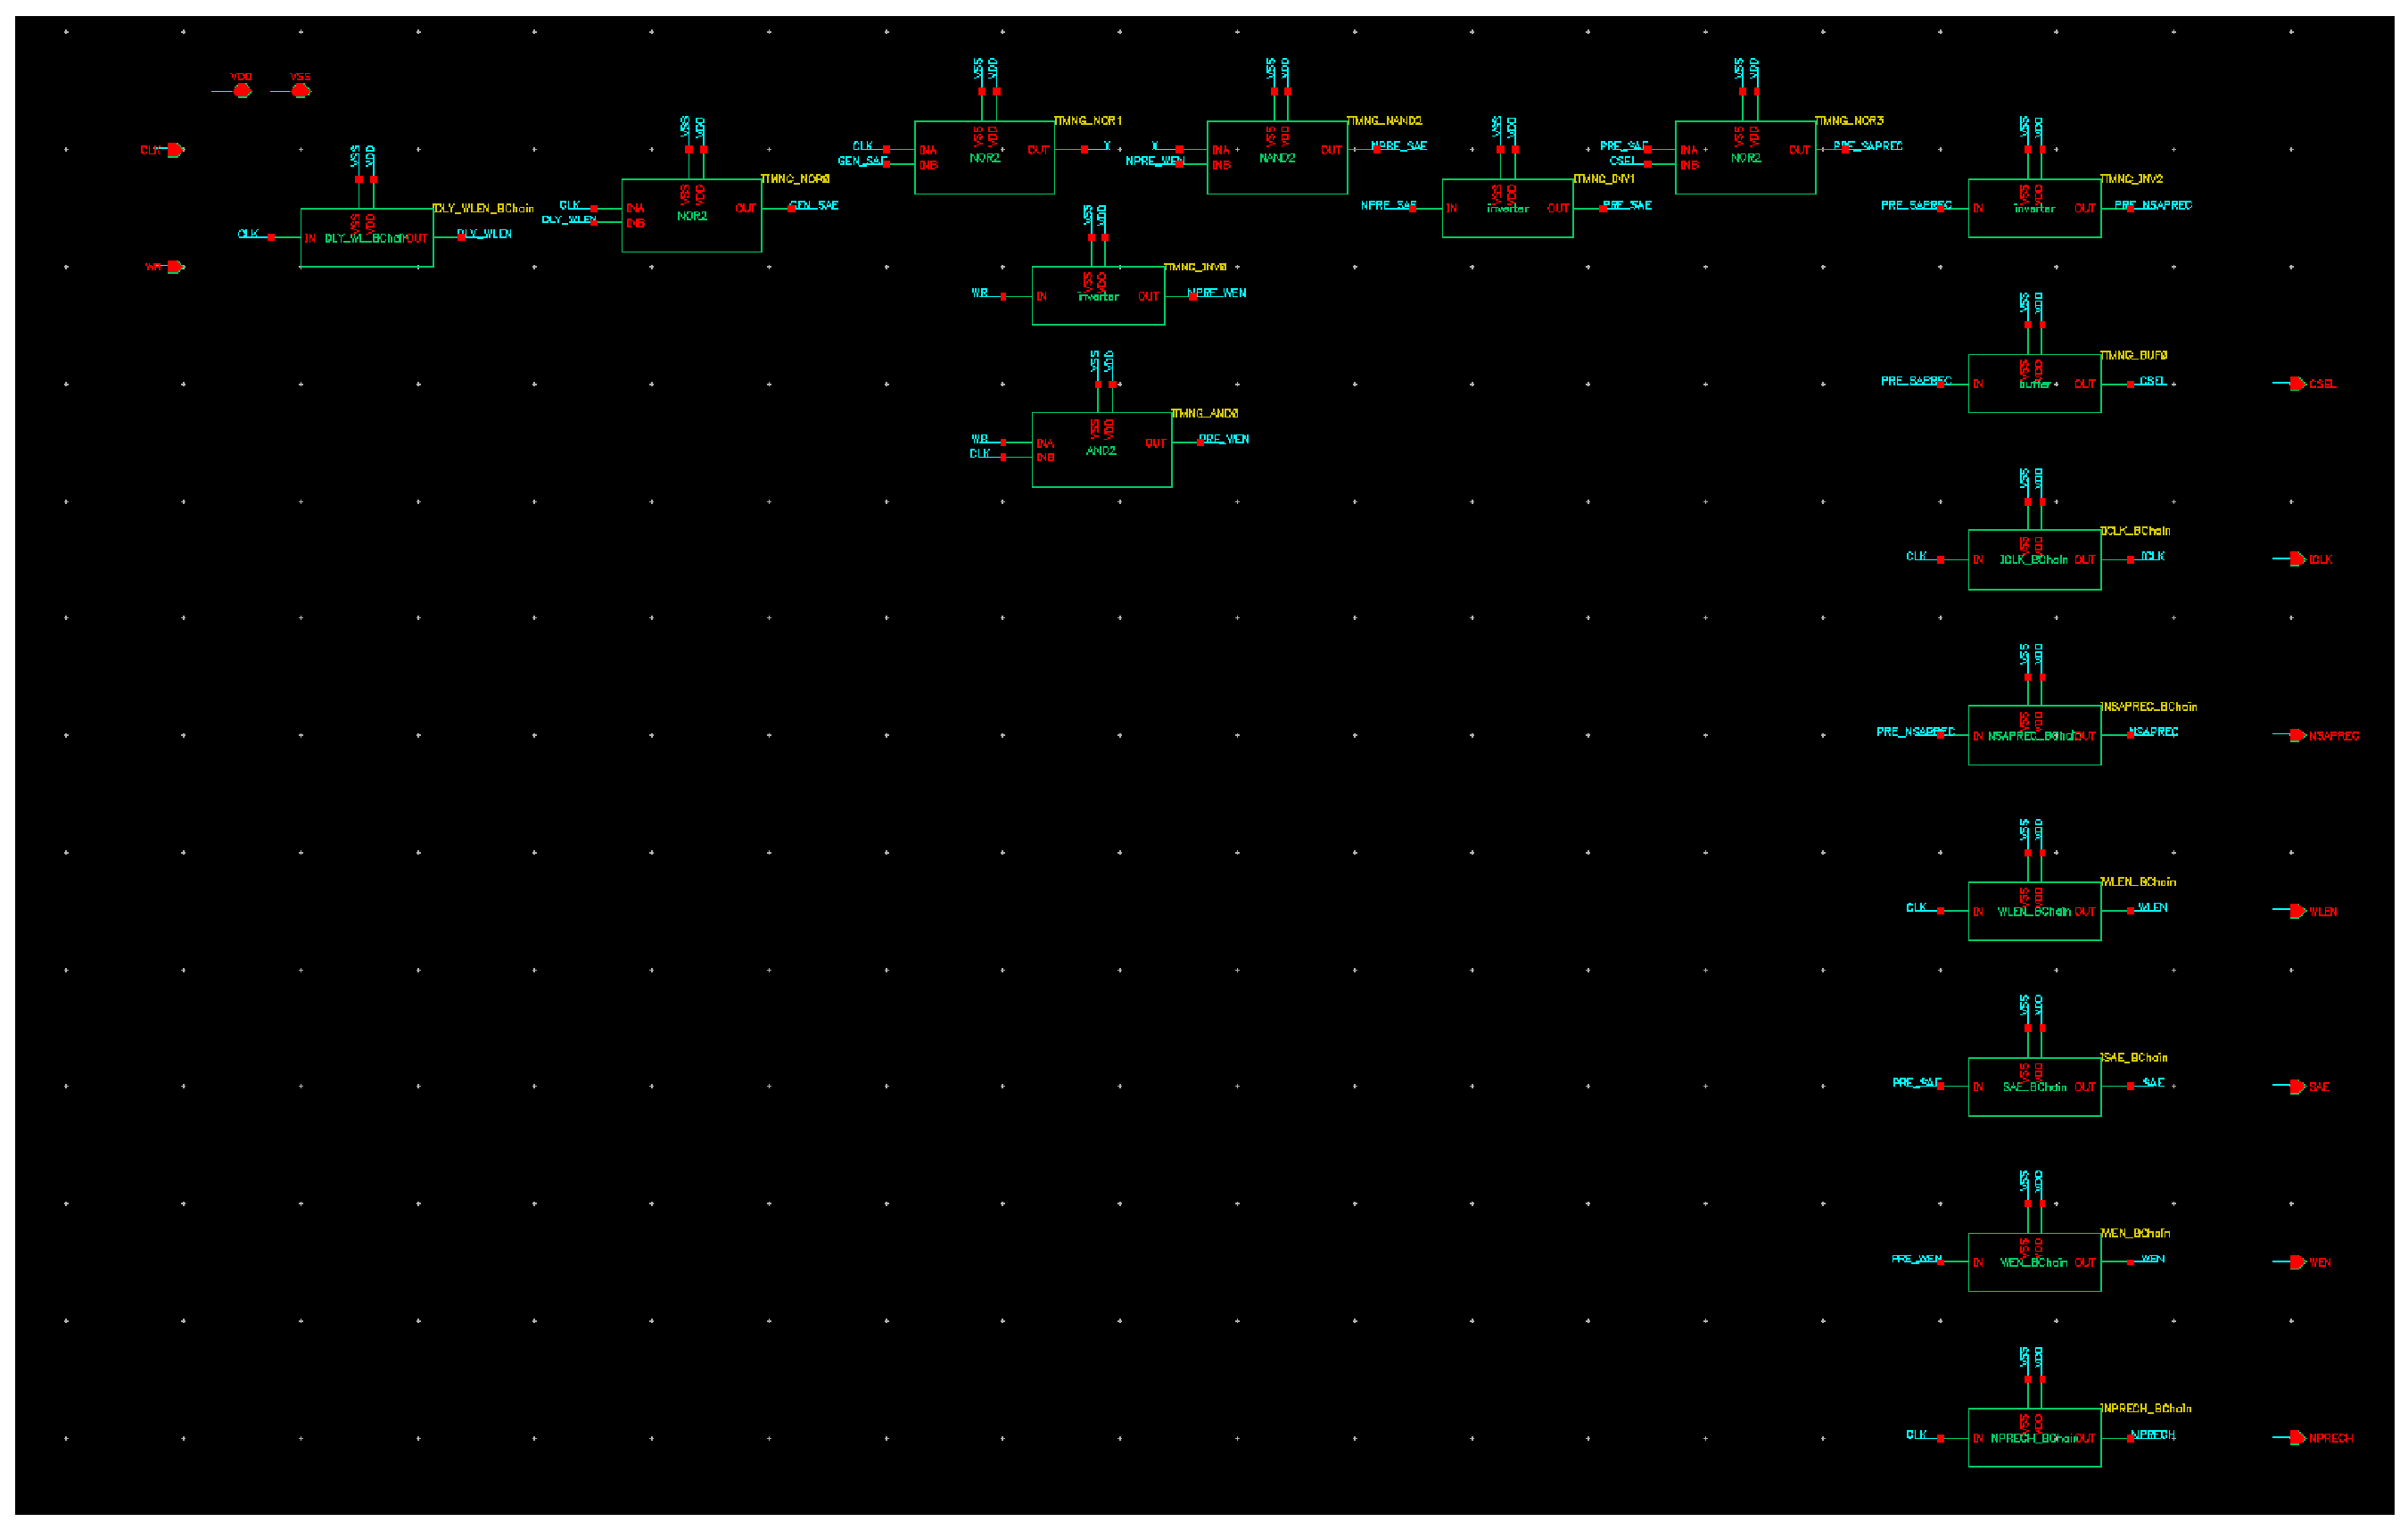
\includegraphics[scale=0.3]{Timing}
\vspace{-5pt}
  \caption{Timing block.}
  \label{fig:tmgblk}
\vspace{-5pt}
\end{figure}

The control signals (listed below), generated for the read and write operations are shown in Figure~\ref{fig:ctrl}. 
\begin{itemize}
\setlength{\itemsep}{0cm}
\setlength{\parskip}{0cm}
\item WEN - Enable for the tri-states in the IO.
\item NPRECH/PCH - BL precharge and equalize transistor control in the CD.
\item NSAPREC/SAPREC - SA precharge control in the SA .
\item CS/CSEL\_i, NCS/CSELB\_i - Column mux transmission gate controls in the CD.
\item SAE - SA enable in the SA.
\item ICLK/OCLK/CLK - CLK signal for different FFs.
\end{itemize}

\begin{figure}[htb]
\centering
\subfigure[]{
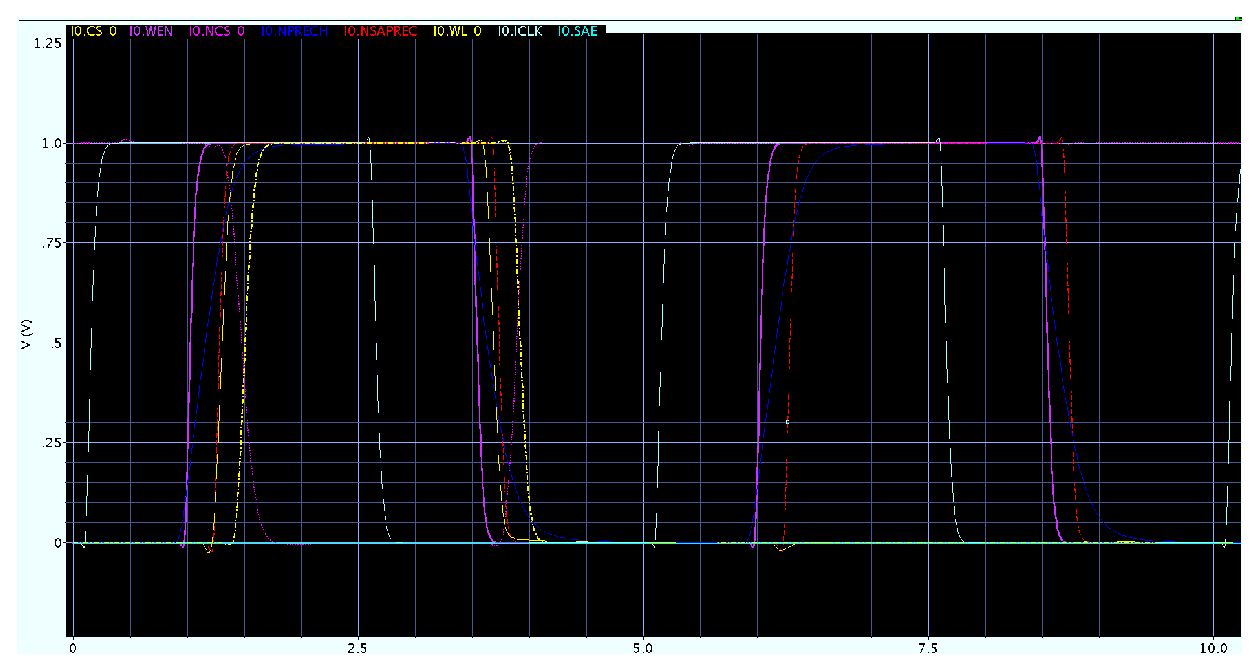
\includegraphics[scale=0.4]{WriteCtrl.eps}
\label{fig:wrt}
}
\subfigure[]{
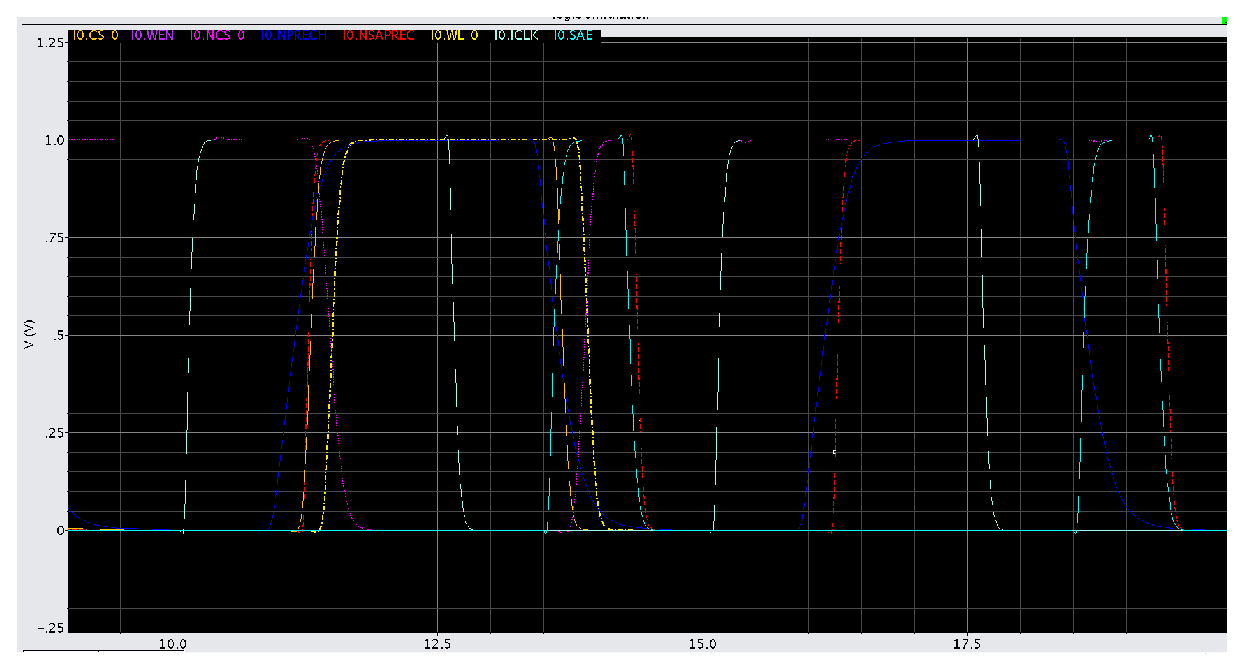
\includegraphics[scale=0.4]{ReadCtrl.eps}
\label{fig:rd}
}
\caption{Timing diagrams showing the control signals for (a) write (b) read}
\label{fig:ctrl}
\end{figure}

The control signals are generated from a clock input to the SRAM, using delay elements. During a write, the control signals (WEN, NPRECH, NSAPREC, CS and NCS) are of the same width and are pulsed some delay after the rising clock edge to allow the address and data inputs to be latched, and to allow the pre-decode and column-decode to finish. The SAE remains low throughout the write cycle. To avoid timing races and to ensure correct functionality, the edges of the pulses should be in the following order (Figure~\ref{fig:wrt}), with an upward arrow indicating a rising edge, and a downward one indicating a falling edge --- WEN$\uparrow$ - NPRECH$\uparrow$ - NSAPREC$\uparrow$ - CS$\uparrow$ - NCS$\downarrow$ - WL$\uparrow$ - WEN$\downarrow$ - NPRECH$\downarrow$ - CS$\downarrow$ - NSAPREC$\downarrow$ - NCS$\uparrow$ - WL$\downarrow$.

During a read, NSAPREC and SAE are not of the same width as the remaining control signals. To ensure that the precharge of the SA inputs is turned off both during the BL differential development, and the SA resolution, the NSAPREC pulse encompasses both these phases. The SAE goes high (e.g. the SA is enabled) towards the end of the WL pulse. The WEN signal remains low throughout the read cycle. The pulse edge order for read is --- NPRECH$\uparrow$ - NSAPREC$\uparrow$ - CS$\uparrow$ - NCS$\downarrow$ - WL$\uparrow$ - SAE$\uparrow$ - CS$\downarrow$ - NCS$\uparrow$ - NPRECH$\downarrow$ - WL$\downarrow$ - SAE$\downarrow$ - NSAPREC$\downarrow$ - ICLK$\uparrow$.

The generation of the control signals can be done using the same logic for any technology. What varies from one technology to another are the characteristics of the buffer chains in the delay elements and the final control signal drivers (e.g. the number of stages, fanout). ViPro can be used to optimize these parameters to ensure proper generation of the control signals in any technology. Section~\ref{sec:opt} discusses the timing optimization in more detail.

\section{Energy and Delay Calculation}
\label{calc}

The devices in each peripheral circuit are parametrized and TASE simulations can determine the E, D characteristics of these circuits across a range of parameters. Both read and write operations can be broken down into two paths --- the circuits between the address and the final WL to the bitcell (Figure~\ref{fig:tmg}), and those driving or receiving the data from the BL(Figure~\ref{fig:col}). Energy and delay or min. cycle time for the SRAM are calculated from the component Es and Ds along these paths, using the following model.
  
\begin{figure}[htb]
  \centering
  \includegraphics[scale=0.35]{Vipro_col}
\vspace{-5pt}
  \caption{A single column and its associated circuitry}
  \label{fig:col}
\vspace{-5pt}
\end{figure}

\subsection{Write}
The minimum cycle time is determined by the critical path delay of the SRAM during a write. The write operation can be broken down roughly into three stages (Figure~\ref{fig:wrtstg}). The first (s1) is the predecode/col-decode and address/data latch stage. The second (s2) is the WL enabled stage where the cell flips. The final (s3) stage is the precharge stage where the BLs are precharged back to prepare for the next access cycle. s3 can occur in parallel with s1 of the next cycle. In sum, the write operation consists of the following actions. 
\begin{enumerate}
\setlength{\itemsep}{0cm}
\setlength{\parskip}{0cm}
\item Input data latching in IO (`io')
\item Row pre-decode (`rowpre')
\item Column decode (`coldec')
\item WL enable (`wld')
\item Bitcell node flip (`bcwr')
\item Precharge BL/BLB (`cdch')
\item Precharge RDWR/NRDWR (`sach')
\end{enumerate}

\begin{figure}[htb]
  \centering
  \includegraphics[scale=0.3]{wrtStg}
\vspace{-5pt}
  \caption{Stages of the write operation}
  \label{fig:wrtstg}
\vspace{-5pt}
\end{figure}

The minimum cycle time for write (T$_\text{MIN-W}$) can be determined as:
\begin{equation}\label{tminw}
\displaystyle  T_{MIN-W}=max(io,rowpre,colpre,cdch,sach) + wld + bcwr
\end{equation} 

If s1 is the bottleneck, s3 of the previous stage can occur in parallel. Thus, a separate pre-charge stage is not required for the write operation and there are effectively only two stages. In this case, the minimum write cycle reduces to 
\begin{equation}\label{tminw}
\displaystyle  T_{MIN-W}=max(io,rowpre,colpre) + wld + bcwr
\end{equation} 

If s3 is the bottleneck, some extra time (s3) is required after s2. The total time available for s3 and the s1 of the next stage should be sufficient to precharge the column. In this case, the minimum write cycle reduces to 
\begin{equation}\label{tminw}
\displaystyle  T_{MIN-W}=max(cdch,sach) + wld + bcwr
\end{equation} 

The energy per access (read or write) is calculated by summing up the energy contributed by each component. The energy is calculated in the following way. First, the average power is measured using-

\begin{verbatim}  
average(getData("<component>:pwr"))
\end{verbatim}

This is the average power measured over the entire simulation time, and does not necessarily correspond to the average power over the actual cycle time. However, the measured energy, which is average power$\times$simulation time will nearly be equal to the actual energy expended in the cycle, except for the leakage energy, which for the peripheral components can be considered to be negligible compared to the switching energy. Thus, we measure the average power and get the energy first by multiplying the simulation time. The top-level SRAM energy is then the sum of the energies of the individual componenets. The top-level SRAM power can now be estimated by multiplying this number with the frequency of operation.

We now briefly discuss the energy calculation during the write operation.
\subsubsection{Bitcell}
The energy dissipated in the bitcell during the write is due to the switching of the storage nodes. As can be seen in Figure~\ref{fig:write_bc}, when the BLs and storage nodes are at opposite values, there is energy dissipated in the bitcell, through the on access transistors. Once the flip nears completion and the V$_\text{DS}$ reduces for the access transistors, the energy goes to zero. The total bitcell write energy can be calculated by multiplying with the number of cells being written, i.e. the word size.

There is also energy dissipated in the half-selected bitcells on the same row, which do a dummy read. This component of the bitcell energy during write can be estimated by multiplying the read energy of the bitcell with the number of unselected columns (i.e. half-selected cell), which is equal to the number of columns minus the word-size.

\begin{figure}[htb]
  \centering
  \includegraphics[scale=0.25]{BC_Write_ptm65}
\vspace{-5pt}
  \caption{Signals and power waveforms for bitcell power during write.}
  \label{fig:write_bc}
\vspace{-5pt}
\end{figure}

\subsubsection{CD}
The CD dissipates power at two points during the write cycle, as seen in Figure~\ref{fig:write_cd}. The first occurs when the column mux trasistors turn on. Energy is dissipated through the transmission gate on the side where the BL is discharging through the PD in the write driver. The BLs are assumed precharged in the sim, so there is no power dissipated by the precharge FET on this side when the WL goes high. The second part of the power dissipation is due to the precharge through the PMOS after the WL has gone low. At this point, the col-mux FETS are off, so the PMOS precharge accounts for the entire power at this point. The total power dissipated in the CD by the accessed columns can be determined by multiplying with the word size as with the bitcell power described above.

The unselected columns have only one component of power dissipation during the write, which is the power dissipated to precharge the bitlines which have drooped due to a dummy read. Multiplying the read CD power (described in the next section) with the number of unselected columns gives the total power.

\begin{figure}[htb]
  \centering
  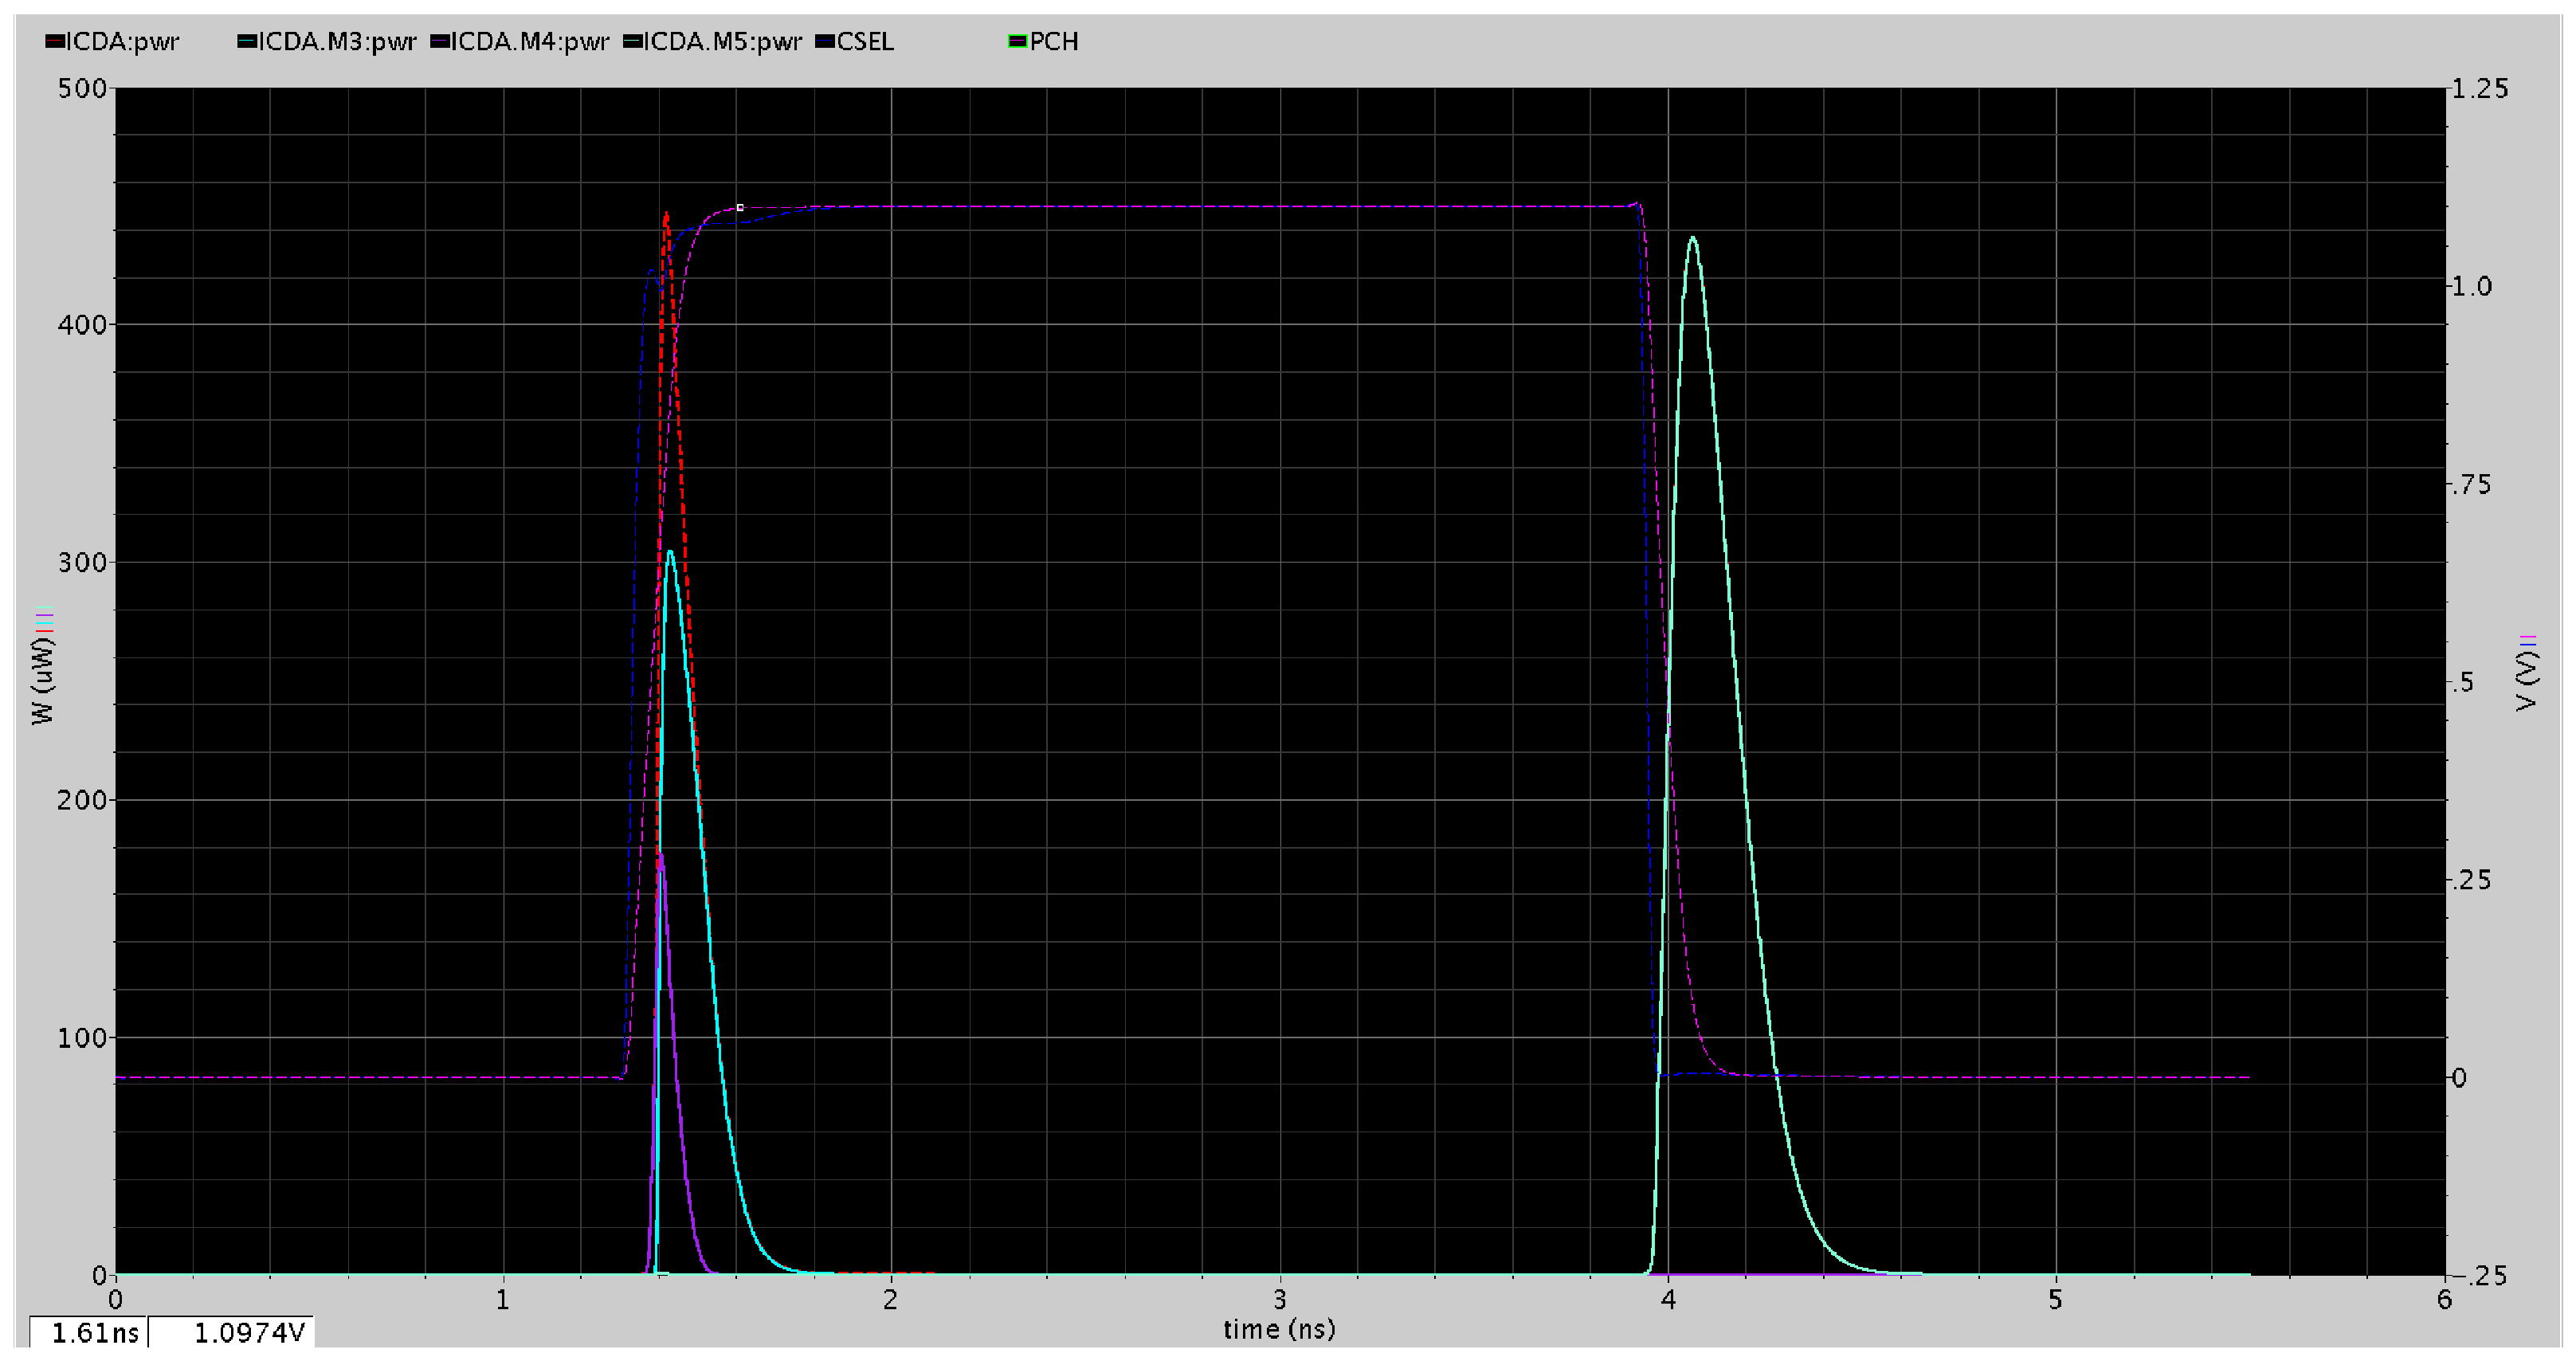
\includegraphics[scale=0.25]{CD_Write_ptm65}
\vspace{-5pt}
  \caption{Signals and power waveforms for CD power during write.}
  \label{fig:write_cd}
\vspace{-5pt}
\end{figure}

\subsubsection{SA}
During the write, since the SA does not sense, the power that is dissipated is due to the pre-charging of one of the NRDWR/RDWR nodes depending on what data was written. Figure~\ref{fig:write_sa} shows the entire power to be due to the precharging of the NRDWR node through the PMOS precharge device. Multiplying the measured power with the word size gives the total power.

\begin{figure}[htb]
  \centering
  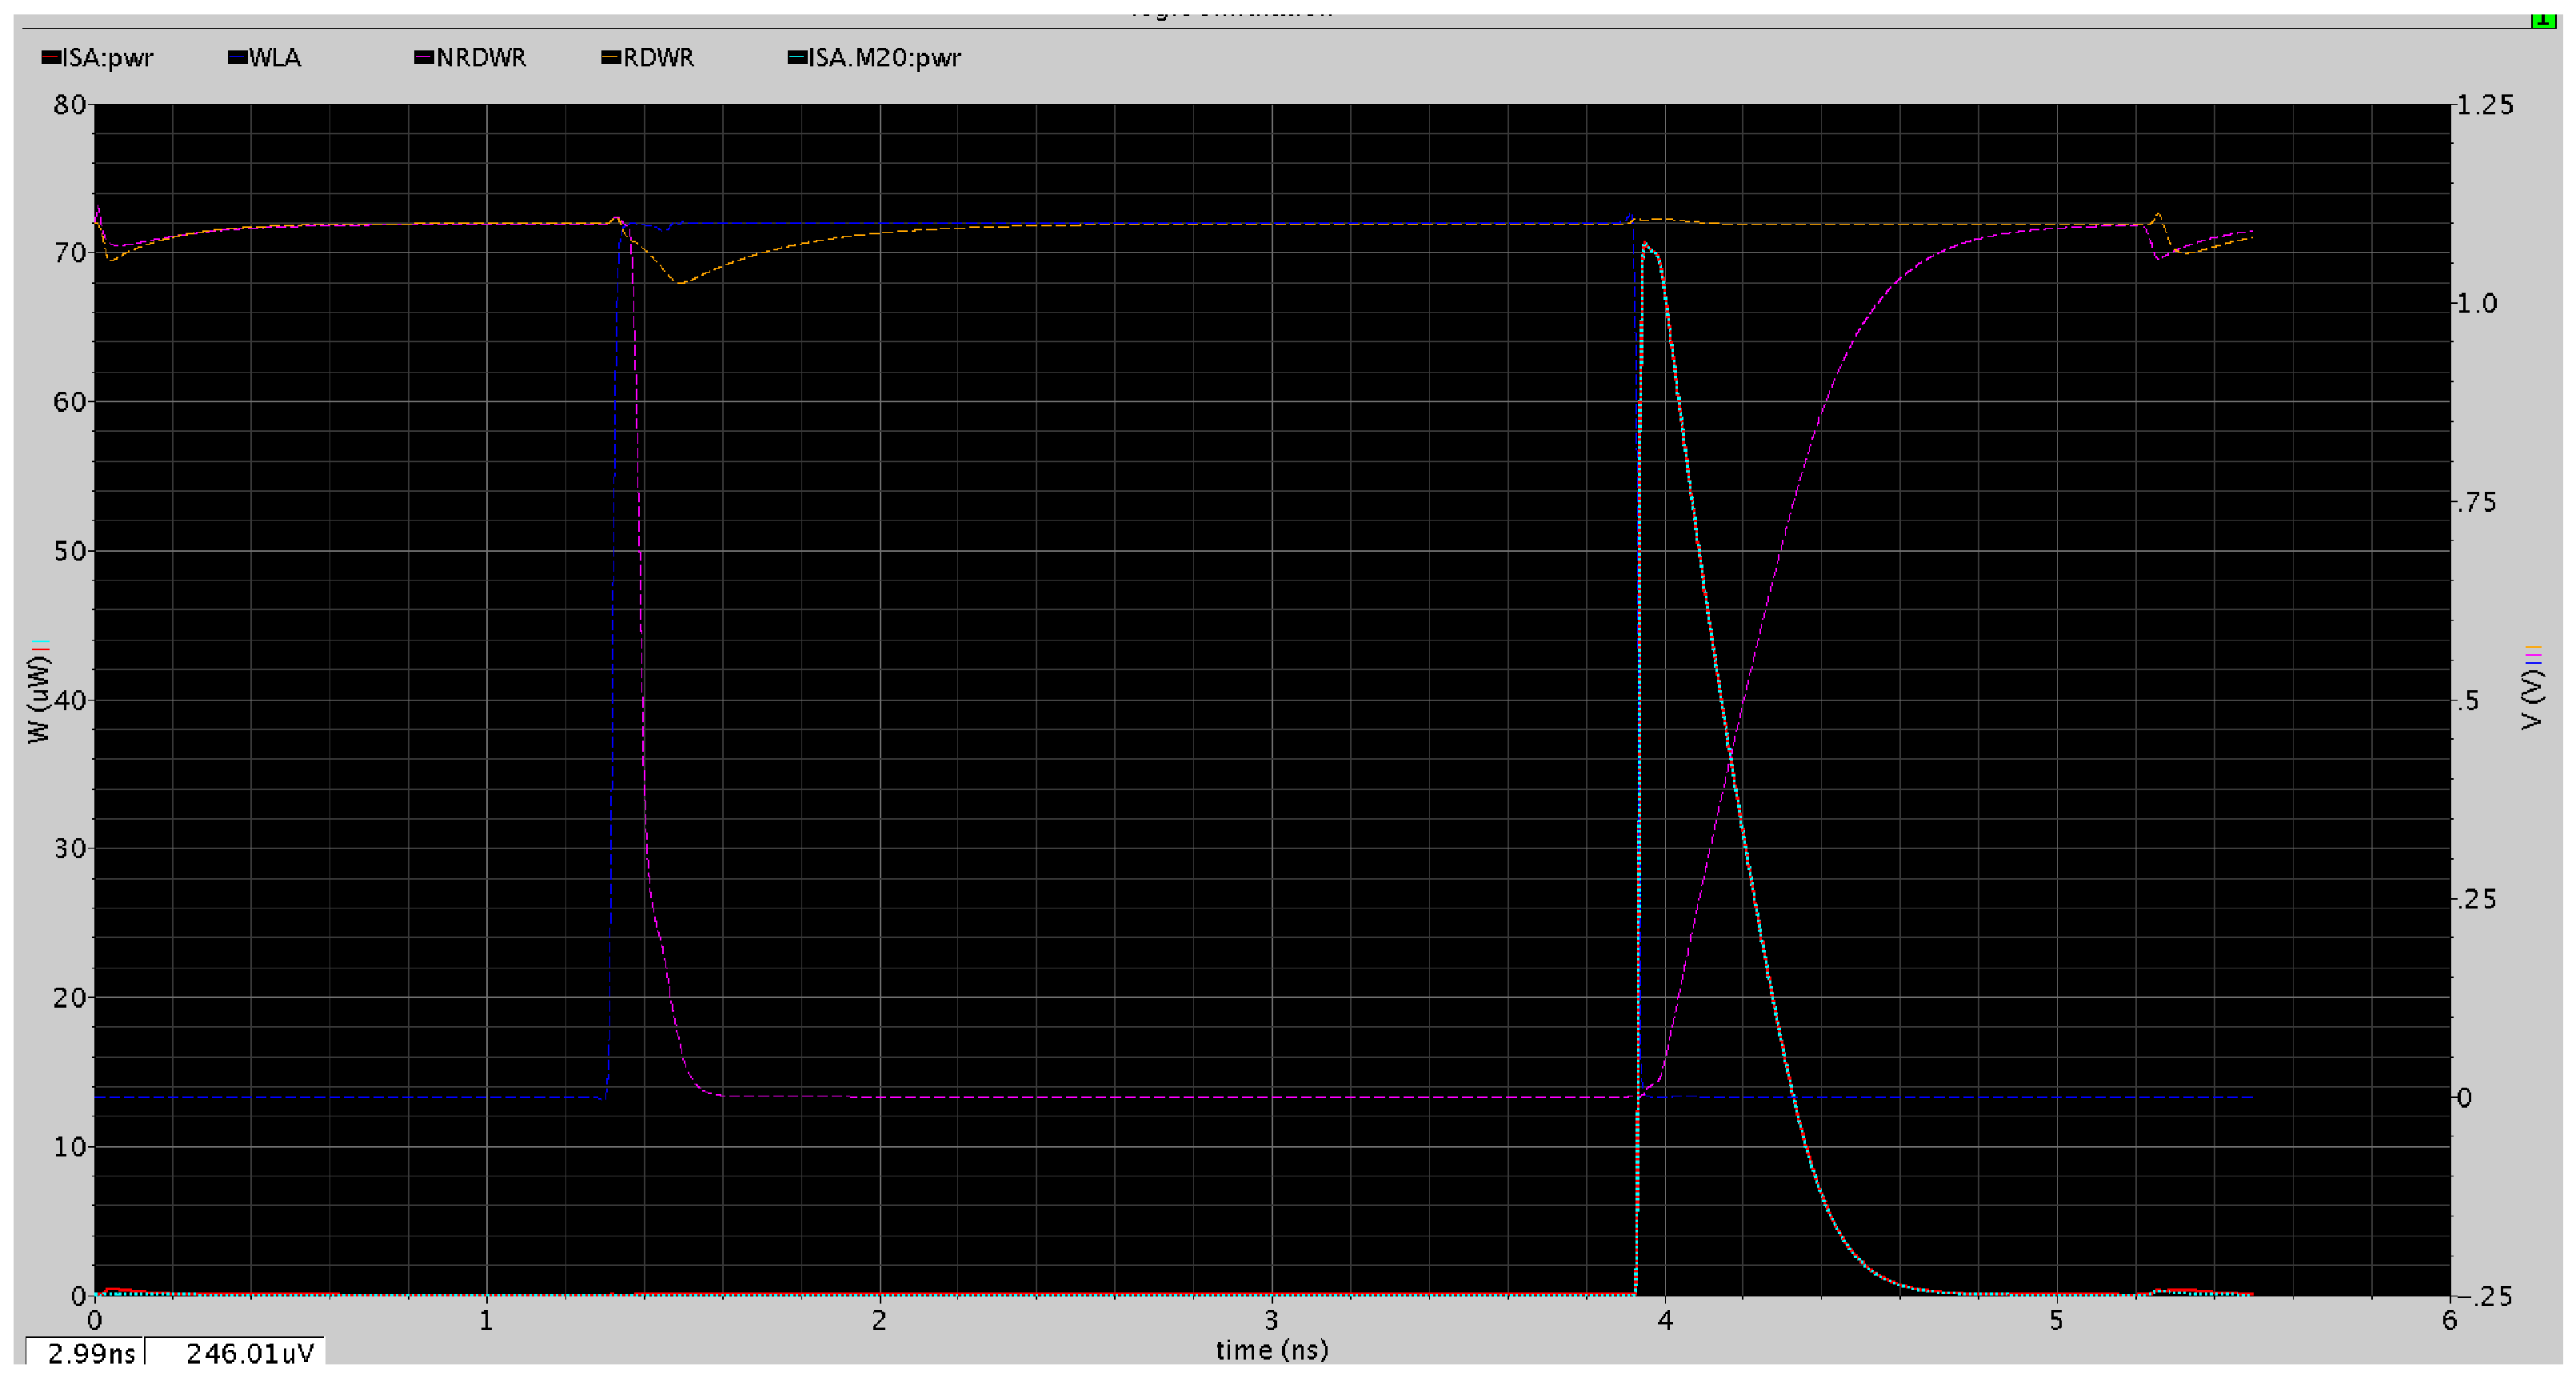
\includegraphics[scale=0.25]{SA_Write_ptm65}
\vspace{-5pt}
  \caption{Signals and power waveforms for SA power during write.}
  \label{fig:write_sa}
\vspace{-5pt}
\end{figure}

\subsubsection{IO}\label{wrtpwr_io}
Figure~\ref{fig:write_io} shows the signals and power waveforms in the IO during a write. There are 4 events that cause power dissipation as can be seen from the figure. First, the rising CLK edge causes both DFFs to consume some power. The Write DFF also consumes power due to latching of the new data value. Consequently, the inverter also flips and contributes to the power at this time. The power consumption of the tri-state inverter driving NRDWR is because one of the PD NFETS turns on when the data gets latched.

Second, when the WEN signal goes high, the tri-state inverters consume power. The RDWR tri-inverter consumes less power since one PD FET turns on while the other turns off, but the PD network of the NRDWR tri-inverter is fully turned on when the WEN signal goes high. So, it dominates the power consumption at this time as one bitline is driven to ground. The other component of power dissipation at this time is due to the switching of the inverters in the WEN buffer.

The third event of power consumption is at the clock falling edge when both DFFs consume power. The final event is when WEN goes low again. At this time the WEN buffer inverters consume power. Also, the first two stages in the write DFF consume power due to the change in the data input at this time.

\begin{figure}[htb]
  \centering
  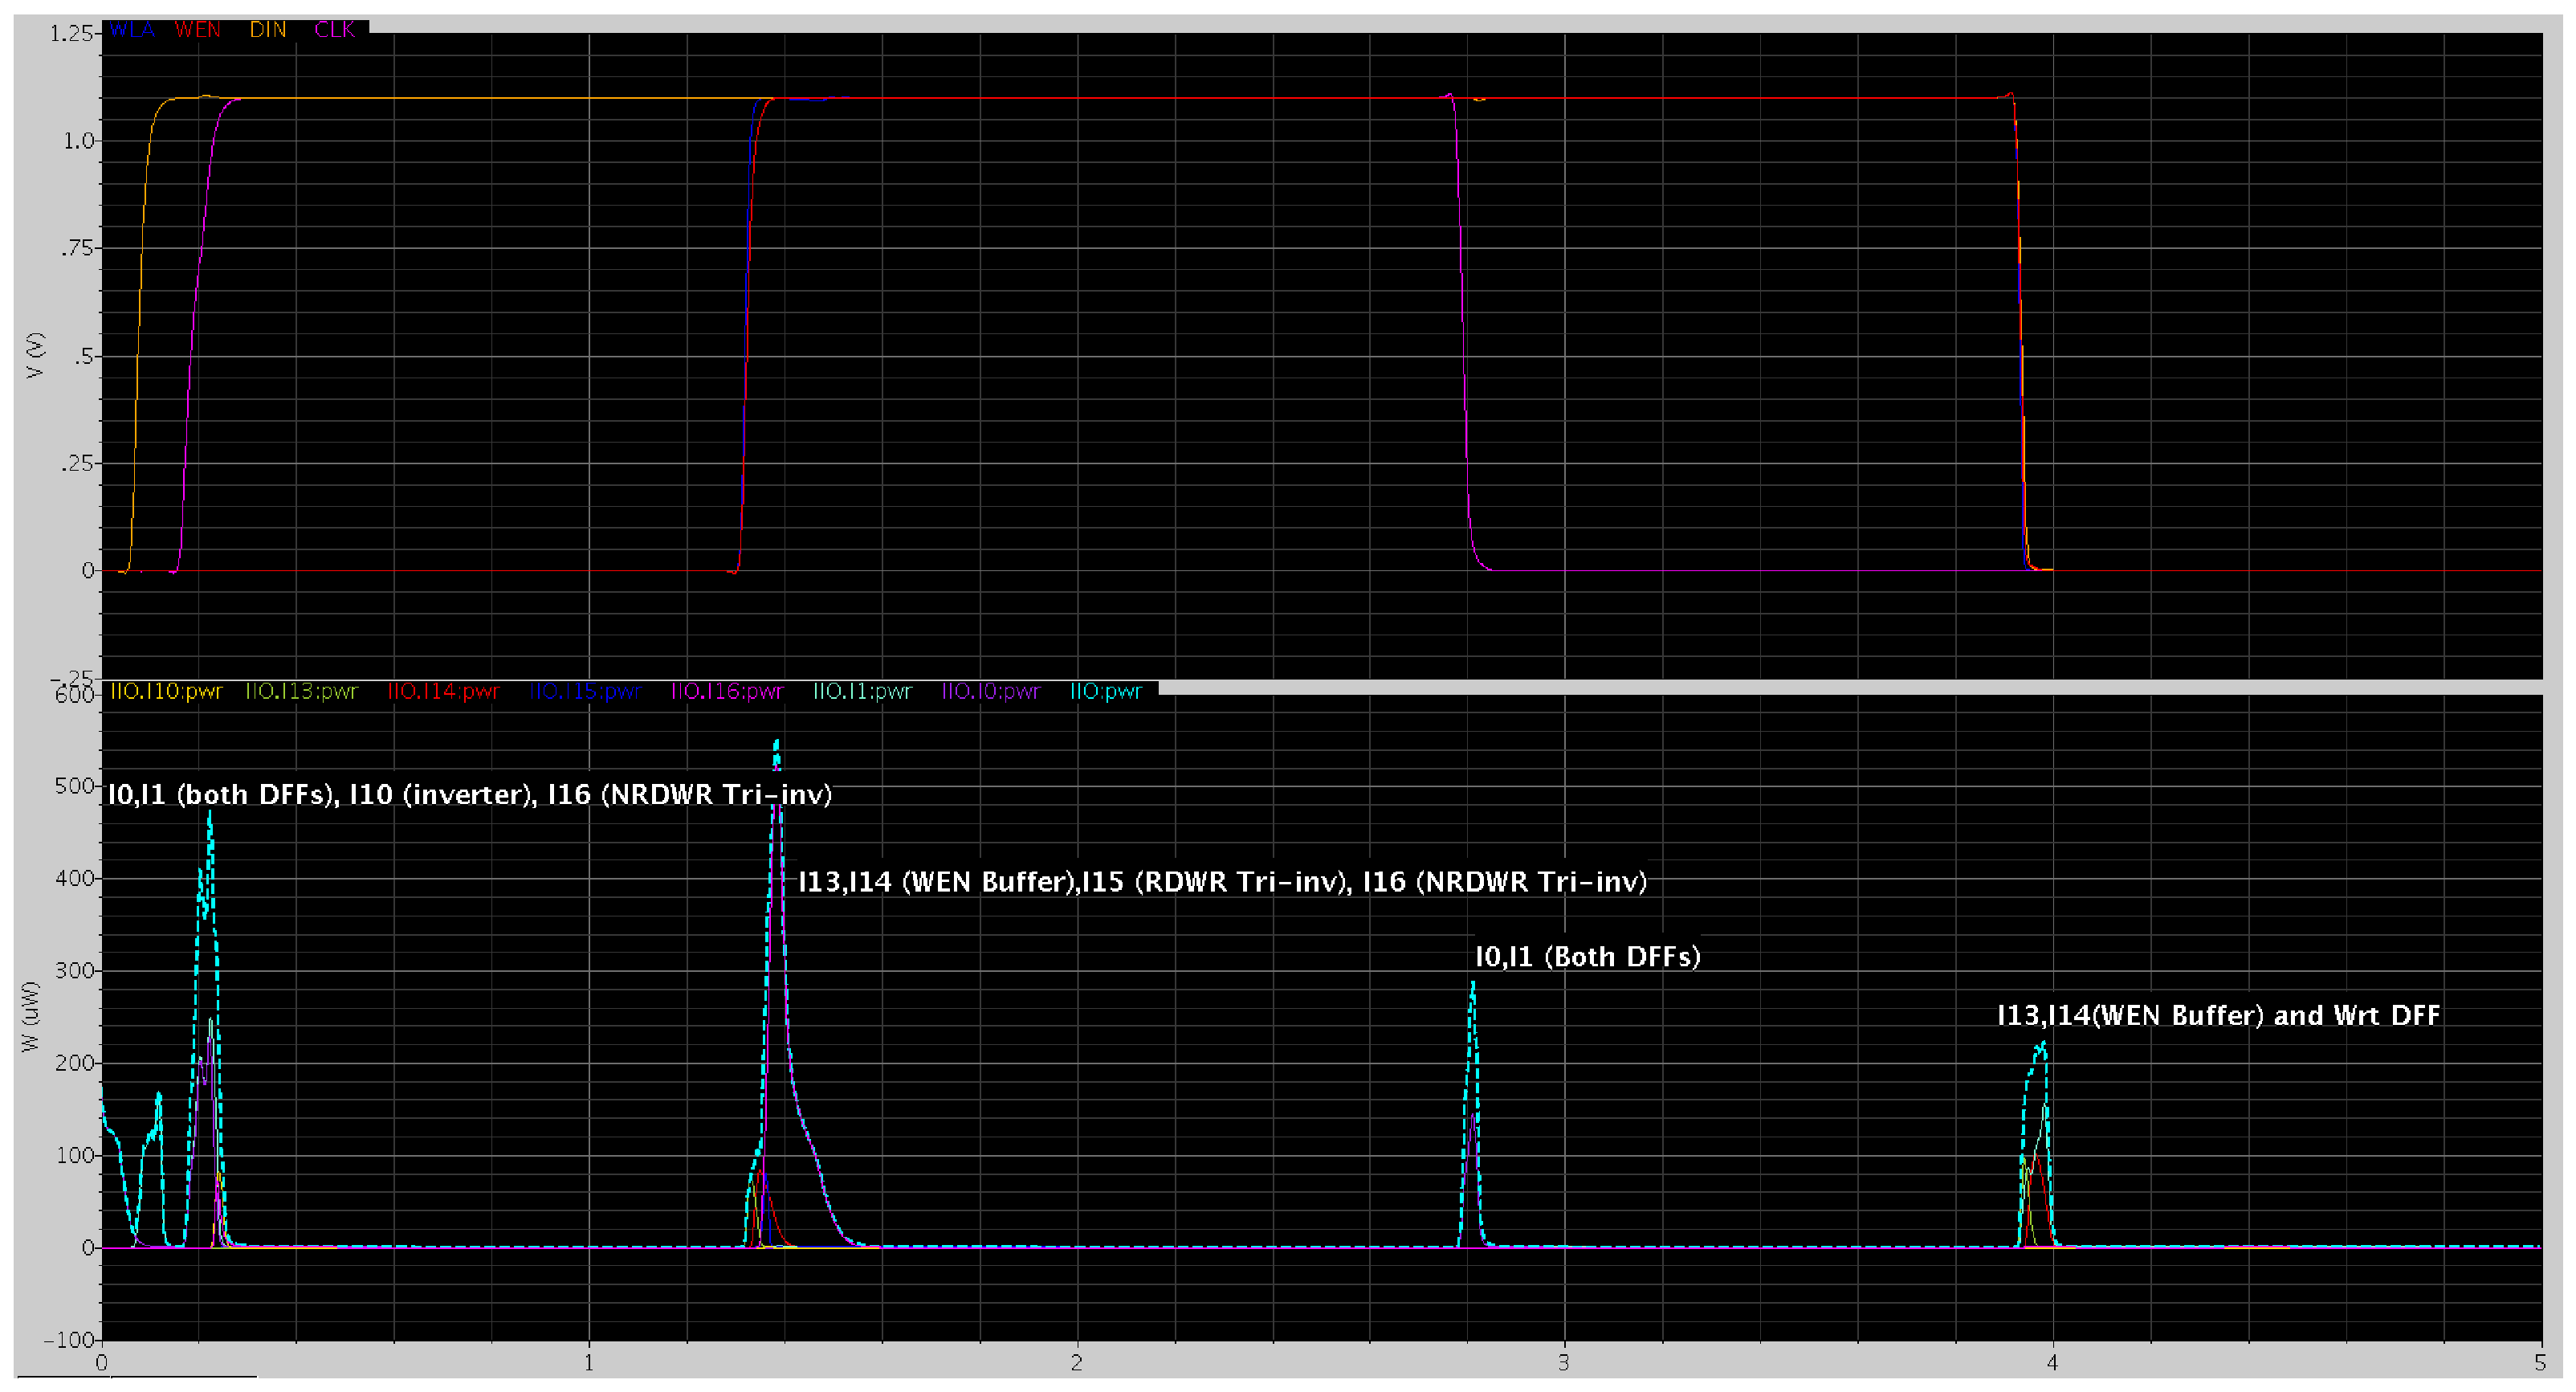
\includegraphics[scale=0.25]{IO_Write_ptm65}
\vspace{-5pt}
  \caption{Signals and power waveforms for IO power during write.}
  \label{fig:write_io}
\vspace{-5pt}
\end{figure}

\subsubsection{Timing}
The average power consumed during write and read is measured. Power is mainly consumed for driving all the control signals horizontally to the bitslice components and vertically to the WL drivers. Since breaking the power down and analyzing it is too complex, we do not describe the timing block power in this document.

\subsubsection{Decoder}
To determine the row decoder and WL driver delays it is sufficient to simulate only the critical path of the decoder. The critical path consists of a predecode phase that drives the vertical predecoded signals to the final decode stage and WL driver that is pitch-matched with each row of the memory. The structure of the critical path varies depending on the number of decoder inputs. We have verified that the power or energy of the critical path is only marginally less (less than 5\%) than that obtained by simulating the whole decoder. So we use the same critical path circuit to determine the energy as well.

The column decoder is a 3 to 8 decoder. The column decoder critical path has a similar gate composition as the 3 to 8 row decoder critical path but for two key differences. One is that there is no intermediate long wire like in the case of the row decoder. The second is the output load being driven by the column decoder, which is composed of the gate caps of the column-mux transmission gates instead of the WL gate capacitances of the bitcells. 

Critical paths for the row and column decoder are shown in Figure~\ref{fig:decCrit}. For the row decoder, buffer chains are tagged on to the end of the predecode and WL driver stages to be able to drive the large capacitances on their outputs. The number of buffer stages in each part of the row decoder is used as a knob in the decoder E-D characterization, as described in ~\ref{subsubsec:decoder}. For the column decoder, the "predecode" is the full 3 to 8 decoder. The second part consists of simply a NAND/AND to combine the decoded output with the column enable signal. The output of this goes to the gates of the column mux transmission gates. The structure of the column decoder critical path is similar to that of a 3 to 8 row decoder with both consisting of only a single NAND/AND in the second (WL Driver) part.

\begin{figure}[htb]
  \centering
  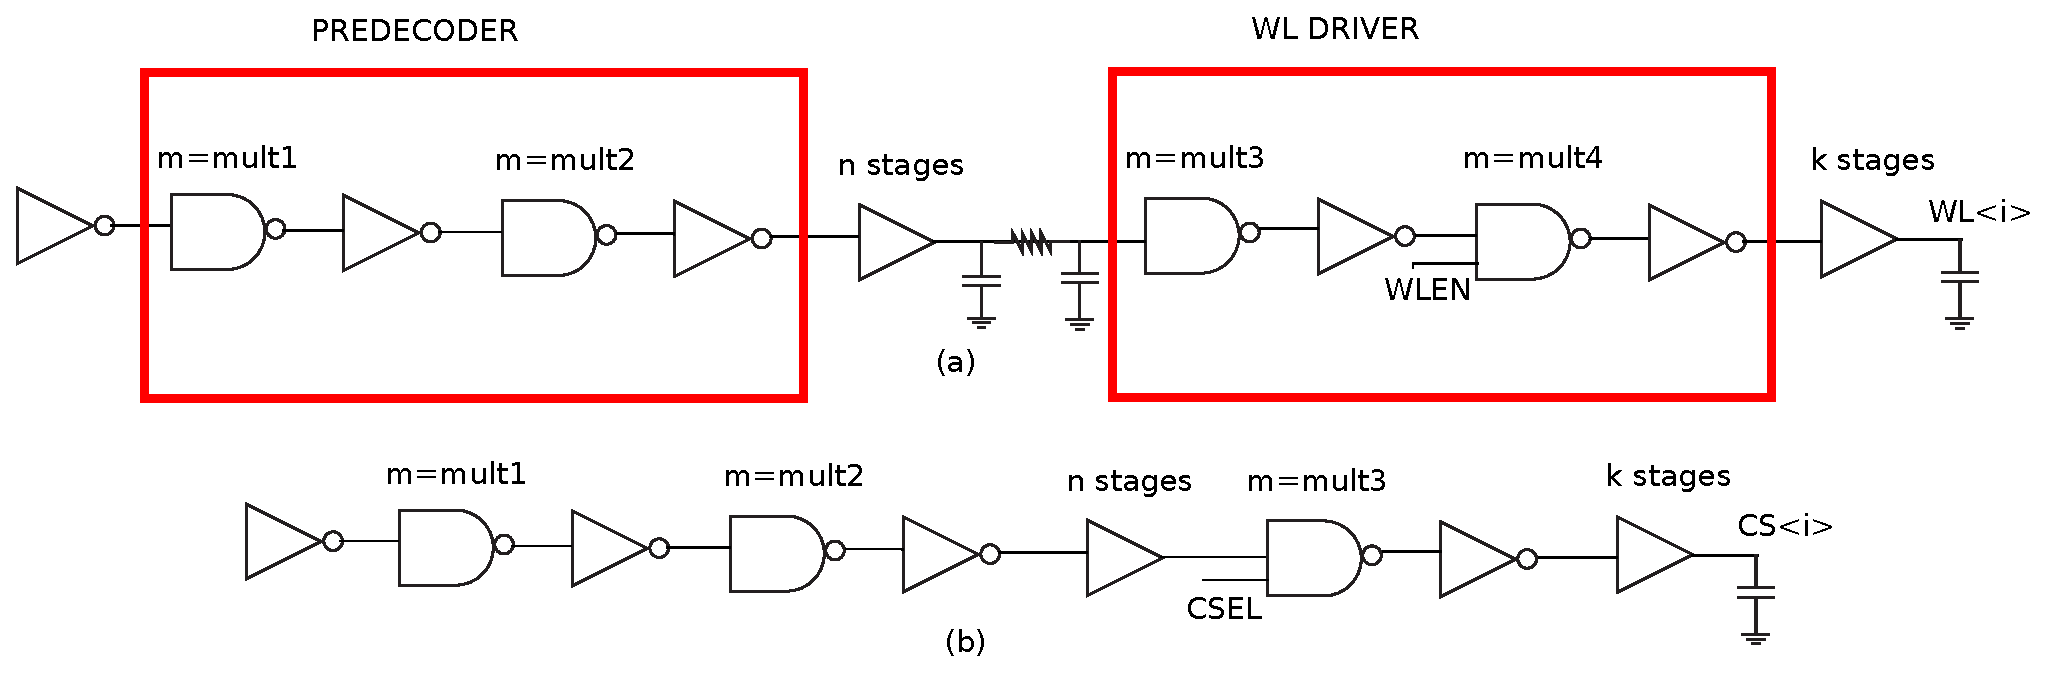
\includegraphics[scale=0.4]{decoder}
\vspace{-5pt}
  \caption{Critical paths for (a)row and (b)column decoder.}
  \label{fig:decCrit}
\vspace{-5pt}
\end{figure}

Figure~\ref{fig:decPower1} shows the power waveforms for various gates in the critical path of the decoder. As Figure~\ref{fig:decPower2} shows, most of the power is dissipated in the final buffer stages of the predecode and the WL driver sections of the decoder since they are big gates driving large load capacitances.
\begin{figure}[htb]
  \centering
  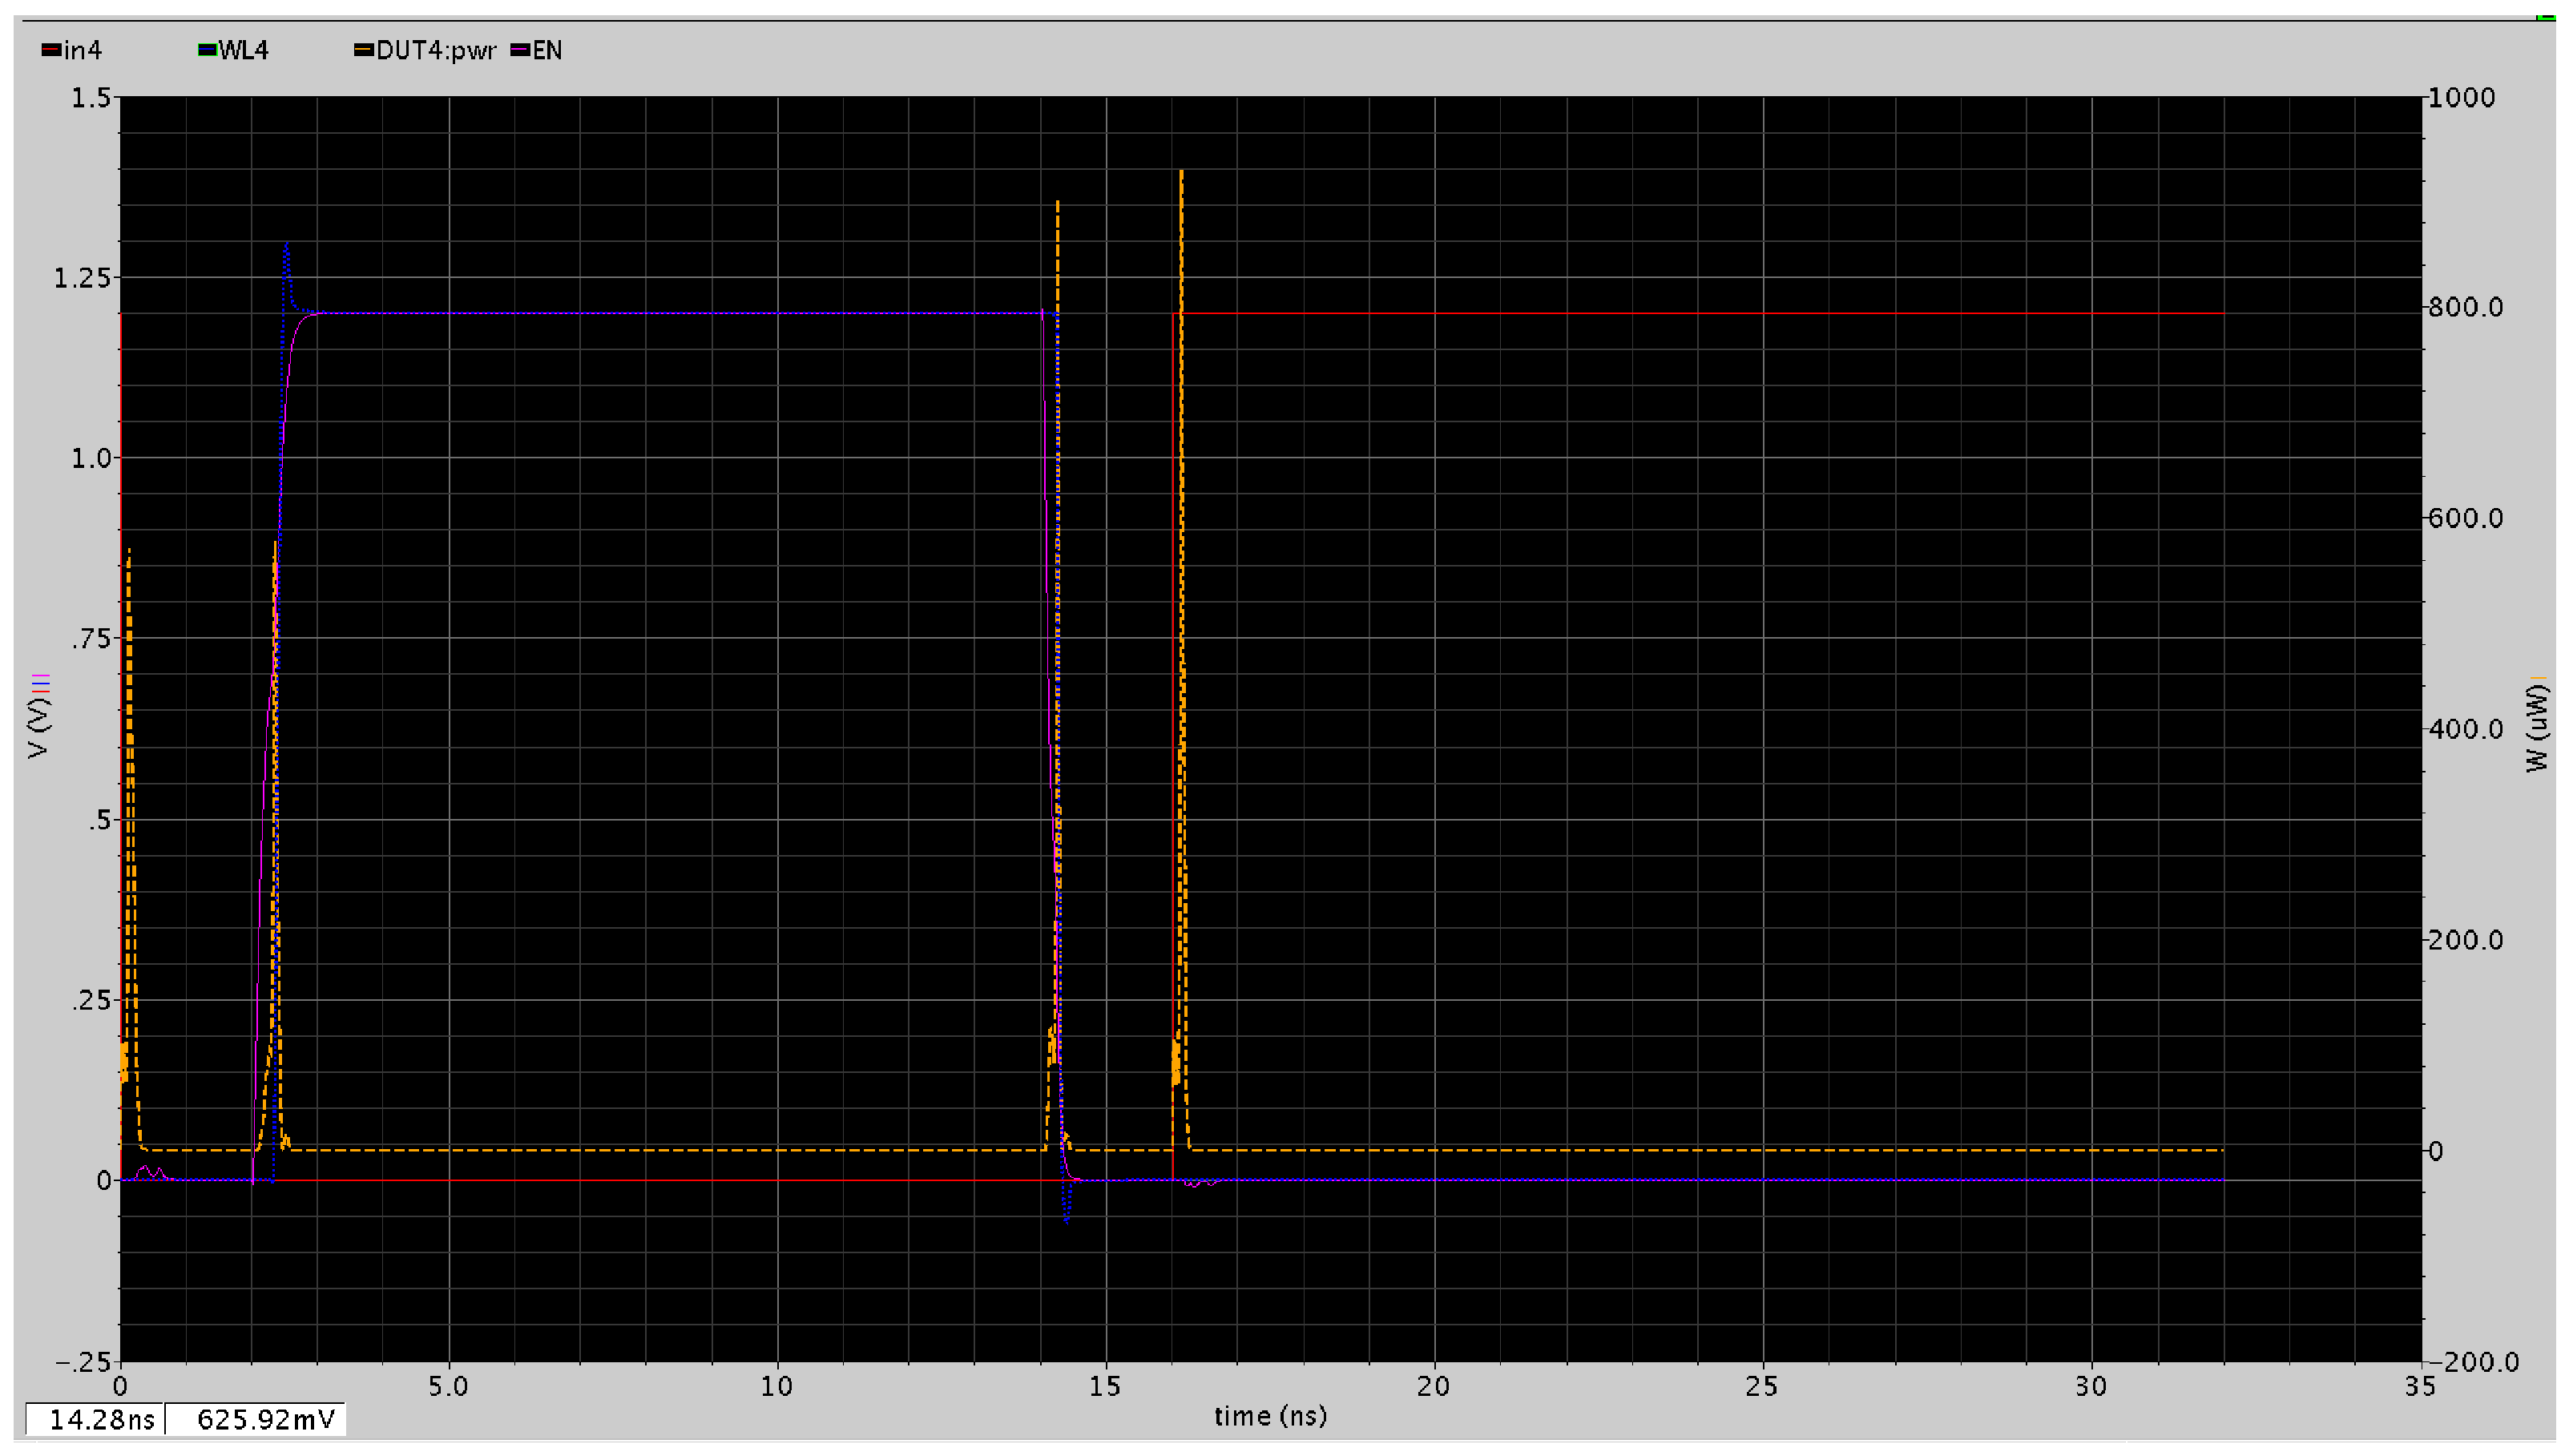
\includegraphics[scale=0.25]{Decoder_power}
\vspace{-5pt}
  \caption{Signals and power waveforms for decoder.}
  \label{fig:decPower1}
\vspace{-5pt}
\end{figure}

\begin{figure}[htb]
  \centering
  \includegraphics[scale=0.25]{DUT4_3bitdecoder_power}
\vspace{-5pt}
  \caption{Power breakup among gates on the decoder critical path.}
  \label{fig:decPower2}
\vspace{-5pt}
\end{figure}

\subsubsection{Leakage}
Only the leakage of the bitcells is considered. The leakage from VDD and VSS and the BL leakage is added to give the leakage of one cell. This is multiplied with the memory capacity to give the leakage of the array. This slightly overestimates the leakage of the array, since the leakage of the bitcells on the accessed row is counted twice - it was accounted for earlier in the dynamic power measurement for the bitcell.

The total energy can now be summarized by the following equation:
\begin{equation}\label{ewrt}
\displaystyle  E_{WRT}=erowpre+ecoldec+ewld+eiowr*ws+(ecdwr*ws+ecdrd*(cols-ws))+esach*ws+(ebcwr*ws+ebcrd*(cols-ws))+etmng+elkg*capacity
\end{equation} 
where
\begin{description}
\setlength{\itemsep}{0cm}
\setlength{\parskip}{0cm}
\item{\textit{erowpre}} = row-predecode energy
\item{\textit{ecoldec}} = col-decoder energy
\item{\textit{ewld}} = WL driver energy
\item{\textit{eiowr}} = IO energy during write
\item{\textit{ecdwr}} = CD energy during write
\item{\textit{ecdrd}} = CD energy during read
\item{\textit{esach}} = SA input/muxed out BL pre-charge energy
\item{\textit{ebcwr}} = bitcell flip energy
\item{\textit{ebcrd}} = bitcell read energy
\item{\textit{etmngwr}} = timing energy during write
\item{\textit{elkg}} = leakage energy
\end{description}

\subsection{Read}
The read operation can be broken down roughly into four stages(Figure~\ref{fig:rdstg}). The first stage,s1, is the same as in the write (e.g. decode). In s2, the WL goes high and the appropriate BL droops due to cell I$_\text{READ}$. In s3, the SA is enabled once a sufficient differential is developed to resolve the BL differential. In s4, the BLs and the SA inputs are precharged back. s4 can occur in parallel with s1 of the next cycle. In sum, the read operation consists of the following actions.
\begin{enumerate}
\setlength{\itemsep}{0cm}
\setlength{\parskip}{0cm}
\item Input data latching in IO (`io')
\item Row pre-decode (`rowpre')
\item Column decode (`coldec')
\item WL enable (`wld')
\item Bitline droop (`bldr')
\item SA resolution (`sa')
\item Precharge BL/BLB (`cdch')
\item Precharge RDWR/NRDWR (`sach')
\end{enumerate}

\begin{figure}[htb]
  \centering
  
\includegraphics[scale=0.3]{rdStg}
\vspace{-5pt}
  \caption{Stages of the read operation}
  \label{fig:rdstg}
\vspace{-5pt}
\end{figure}

The minimum cycle time for read (T$_\text{MIN-R}$) can be determined as:
\begin{equation}\label{tminr}
\displaystyle  T_{MIN-W}=max(io,rowpre,colpre,cdch,sach) + wld + bldr + sa
\end{equation} 

The setup time for the flip-flop that latches the output of the SA must also be added to this delay. Since that is quite small (Figure~\ref{fig:tsu}) compared to the other terms in equation \ref{tminr}, we ignore it.

\begin{figure}[htb]
  \centering
  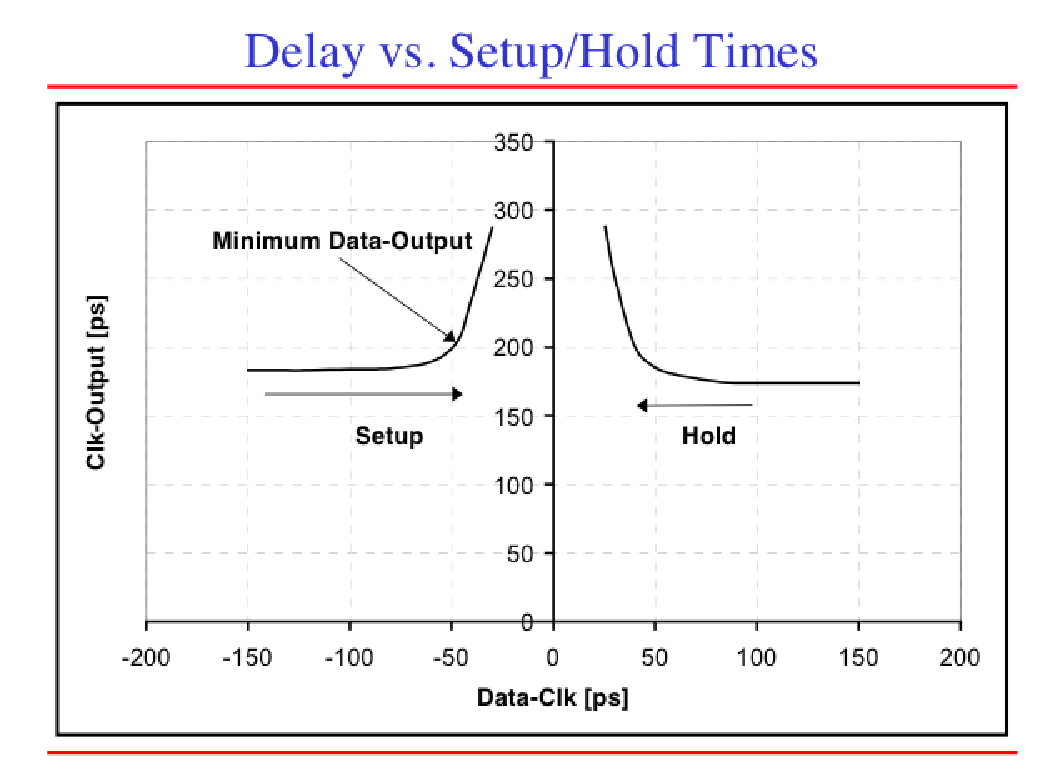
\includegraphics[scale=0.5]{tsu_th}
\vspace{-5pt}
  \caption{Setp and Hold time}
  \label{fig:tsu}
\vspace{-5pt}
\end{figure}

We now discuss the energy components during a read.

\subsubsection{Bitcell}
During a read, the power dissipated through the bitcell is in the PD and PG of the bitcell that are discharging the BL, as shown in Figure~\ref{fig:read_bccd}. 
\begin{figure}[htb]
  \centering
  \includegraphics[scale=0.25]{BC_CD_Read_ptm65}
\vspace{-5pt}
  \caption{Signals and power waveforms for CD and bitcell power during read.}
  \label{fig:read_bccd}
\vspace{-5pt}
\end{figure}

\subsubsection{CD}
During a read, the power dissipation in the CD is only due to the precharging of the partly discharged BL back to full rail V$_\text{DD}$, as can be seen in Figure~\ref{fig:read_bccd}. Unlike in the write operation, there is no significant power dissipation in the CD at the beginning of the WL pulse since both the BL and the RDWR/NRDWR nodes are precharged high and there is no significant current through the column-mux transmission gates.

\subsubsection{SA}
There are two main power dissipation sources in the SA during a read, as observed from the waveforms in Figure~\ref{fig:read_sa}. The first component is due to the resolution of the BL differential by the SA. The second part is due to the pre-charging of the SA inputs(e.g. RDWR/NRDWR nodes).

\begin{figure}[htb]
  \centering
  \includegraphics[scale=0.25]{SA_Read_ptm65}
\vspace{-5pt}
  \caption{Signals and power waveforms for SA power during read.}
  \label{fig:read_sa}
\vspace{-5pt}
\end{figure}

\subsubsection{IO}
During a read, the IO power dissipation is predominantly due to the DFFs since the the write drivers are inactive. There are two power consumption events as seen from Figure~\ref{fig:read_io}. These correspond to the rising and falling edges of the clock during which the DFFs consume power. The latching of the SA output data also occurs at the rising edge adding to the power consumption.

\begin{figure}[htb]
  \centering
  \includegraphics[scale=0.25]{IO_Read_ptm65}
\vspace{-5pt}
  \caption{Signals and power waveforms for IO power during read.}
  \label{fig:read_io}
\vspace{-5pt}
\end{figure}

\subsubsection{Decoder, Timing, Leakage}
The Decoder power consumption and the leakage are the same during write and read and is as described earlier. A single timing block characterization is used to calculate the average power for both read and write as described earlier.

To get the total energy for the IO,CD,SA, and bitcell, we multiply the energy measured from the TASE sim with the word-size as before. The energy per read access can be calculated as:
\begin{equation}\label{erd}
\displaystyle  E_{RD} = erowpre + ecoldec + ewld + eior + ecdrd + esa + ebcrd + etmngrd + elkg
\end{equation} 

\begin{description}
\setlength{\itemsep}{0cm}
\setlength{\parskip}{0cm}
\item{\textit{esa}} = SA energy during read
\item{\textit{etmngrd}} = Timing energy during read
\item{\textit{eior}} = IO energy during read
\end{description}

\section{Optimization}
\label{sec:opt}
\subsection{Knobs for optimization}
To simplify the optimization problem and manage complexity we restrict ourselves to a subset of design variables that can be tuned to generate an optimal SRAM virtual prototype that fits the user constraints. In this section, we describe our choice of knobs for optimization for each subcomponent.

\subsubsection{Bitcell}
For the basic case of a super-threshold, 6T SRAM, we use the bitcell provided in the design kit by the foundry. This bitcell is already carefully designed and optimized for area, power and performance and to simplify the problem we use this bitcell as is. For other kinds of SRAM, e.g. sub-vt, alternative bitcells etc., a bitcell is generated by the bitcell generator.

\subsubsection{CD}
The design variables that can influence the E and D of the CD are the device dimensions of the precharge, equalize, transmission gates, number of rows (NR) and V$_\text{DD}$. We assume the lengths of all devices to be the minimum/default length for the technology. We also make the width of the PMOS and NMOS in the transmission gate the same, as there is no need to balance the drives of each. We make the equalize transistor the same size as the precharge so that we have a uniform rectangle in the layout for the two PMOS and equalize transistor. Thus the variables are now reduced to the widths of the various transistors, NR, and V$_\text{DD}$.

By running the CD\_sizing test in device/TESTS, we find that the energy contribution of the precharge or the pass gate transistor does not change much for a given BL capacitance if it is upsized. This is because the load capacitance remains more or less constant as it is dominated by the BL capacitance. Thus energy is not a consideration when trying to size these devices. So we just upsize these devices till the delay lies on the knee of the delay-width pareto curve. For different technologies and for various values of BL capacitance, we find that a sizing of about 5-6 times the minimum width is optimal for these devices. This ensures the precharge is fast enough so it does not lie on the critical path during read while not being too area hungry. Also keeping these devices small helps reduce the load on the buffers in the timing block that drive the control signals to the gates of the precharge and transmission gates (e.g PCH, CSEL etc.).

Thus, in sum, the knobs for the CD are NR and V$_\text{DD}$, which are also global knobs that influence other component ED characteristics. All device lengths are the minimum values and all device widths are 6$\times$ the minimum. 

\subsubsection{SA}
The SA contribution to the total energy is not very significant. The SA design is based mainly on the failure probability. Using Mahmoodi's paper on sizing each device in the SA and how it affects the failure probability of the SA, we determine the sizes of the devices in the SA. 

First, we make the precharge and equalize transistors for the output nodes (OUT/OUTB), and the internal evaluation node (xin/xinb) minimum sized since these are small capacitances. The PFETs in the cross-coupled inverters are also minimum sized to reduce failure probability as is the NMOS footer. The NFETs in the cross-coupled inverters are made 3$\times$ the minimum width to reduce failure probability. This is the device that most affects the failure probability. The input NFETS that are driven by the RDWR/NRDWR also reduce the failure probability if they are upsized, but not as significantly as the cross-coupled NFETs do. So, we leave them minimum sized. Finally, the precharge PFETs for the RDWR/NRDWR are made 5$\times$ the minimum width as we did for the CD. Here we assume that the capitance being driven by these FETS is large compared to the self-load, since this node has the SA input, the CD transmission gate, the IO driver, and the long RDWR/NRDWR wire.

\subsubsection{Decoder}
\label{subsubsec:decoder}
The decoder E-D characteristics are influenced by the gate sizing, V$_\text{DD}$, and number of stages in the predecode and WL buffer chains. The knobs we use are the number of buffer chain stages and V$_\text{DD}$. We assume that the first gate of the buffer chain is minimum sized and the fan-out if 4, which is a good heuristic to reduce energy while paying only a small delay penalty (ref - Amrutur and Horowitz, Fast low-power decoders for SRAM). The optimal number of stage increases as the output WL load or the predecode wire load increases.

\subsubsection{Timing}
The timing block E-D are influenced by the buffer chains that drive the horizontal control and vertical predecode lines. The characteristics (e.g. sizing, number of stages) of these chains depend on the load that they are driving which depends on the number of rows/columns. So, this is one knob. The second knob is V$_\text{DD}$.

\section{Compiler}
\label{sec:compiler}

The compiler in ViPro consists of technology agnositic schematic and layout generators. These are described in the following subsections.

\subsection{Schematic Generator}
compiler/schematic contains the SKILL scripts used to generate the SRAM schematic. The top-level wrapper script is darUvaEceSRAM\_Schematic.il. It takes 3 files as inputs - inputs.txt, minSizes.txt, and sizes.txt. First, the basic gates are generated. Next, the leaf nodes, such as WL drivers, SA, CD etc. are generated. Finally, these are hierarchically tiled to generate the full SRAM schematic.

To generate an SRAM schematic in a new technology, follow these steps.
\begin{enumerate}
\setlength{\itemsep}{0cm}
\setlength{\parskip}{0cm}
\item Add the technology template directory (template/\textless technology \textgreater/) with the include.scs, subN.scs and subP.scs files.
\item Add the RVPtpl\_ \textless technology \textgreater .ini file to the template/ directory.
\item Modify configuration/user.m and configuration/bitcellSizes.m. 
\item Run the following command. "perl ViPro.pl --clean --char". This will create ctrlBufChains\_*.txt in the files/ directory.
\item Create "optParams.txt" file in the files directory. This file currently looks like this:
\begin{verbatim}
decoder 9 1 1
ctrlBuf 4	5	4	3	3   4.34	4.48	4.14	7.41	6.24
\end{verbatim}
The first line specifies the number of row address bits, the number of predecode \textit{buffers}, and the number of WL \textit{buffers}. The second line specifies the number of \textit{inveter} stages and fanout for the buffer chains corresponding to the timing block signals going to the bitslice (CSEL, NPRECH, NSAPREC, SAE, WEN). These numbers can be got from files/ctrlBufChains\_*.txt from the line corresponding to the required column-muxing.

Through these steps ViPro should ensure a working SRAM. The user only needs to select sufficient number of decoder buffer stages in the first line of optParams.txt. Eventually, the idea is for optParams.txt to be generated automatically from the optimization.
\end{enumerate}

\subsection{Layout Generator}
The layout generator is currently hard-coded for a particular technology (st65). It tiles together manually created leaf node layouts to first create the WL driver, bitslice, and the array. These blocks are then abutted together with the timing block (assumed synthesized) to generate the layout of the SRAM.

Eventually, the idea is to use pycell to create at least the leaf layouts for any technology. Then, either SKILL or pycell itself can be used again to hierarchically create the top-level SRAM layout.


\section{Trouble-shooting tips}
If things are not working, one or more of the following things may be the reason.

\begin{enumerate}
\item Configuration error - One or both of user.m and bitcellSizes.m could be absent, missing some mandatory parameters, or have wrong parameters.

\item Flag error - Make sure that the right flags are provided. For example, the --char needs to be use at least once for each technology to produce the TASE characterization data. 

\item TASE failure - The characterization step can fail for a number of reasons - 
\begin{itemize}
\setlength{\itemsep}{0cm}
\setlength{\parskip}{0cm}
\item Environment setup
\item Model file path
\item Simulation setup
\item Matlab
\item LaTeX
\end{itemize}
For more details on these and ways to debug and fix TASE problems, refer to the TASE user guide.

\end{enumerate}

\input{functions}
% \vspace{6pt}
% \noindent {\bf Categories and Subject Descriptors:} B.7.1 [Integrated circuits]: Types and Design Styles---Advanced technologies
% \terms{Algorithms}
% \noindent {\bf General Terms:} Design, Performance, Reliability
% \keywords{Model-order reduction, skin effect, interconnect}
% \noindent {\bf Keywords:} Graphene nanoribbons, variability, defects

%\scriptsize{
%\bibliography{ViPro_UG}
%\bibliographystyle{ieeetr}}

\end{document}
%--that's it------------------------------------------------
